% !TEX program = pdflatex
%  LaTeX support: latex@mdpi.com

%=================================================================
\documentclass[applsci,article,submit,pdftex,moreauthors]{Definitions/mdpi}

%=================================================================
% MDPI internal commands - do not modify
\firstpage{1}
\makeatletter
\setcounter{page}{\@firstpage}
\makeatother
\pubvolume{1}
\issuenum{1}
\articlenumber{0}
\pubyear{2026}
\copyrightyear{2026}
\datereceived{ }
\daterevised{ }
\dateaccepted{ }
\datepublished{ }

%=================================================================
% Custom commands and packages
\newcommand{\dotmH}{\dot{m}_{H_2}}
\newcommand{\dotmmin}{\dot{m}_{H_2,\text{min}}}
\newcommand{\dotmopt}{\dot{m}_{H_2,\text{opt}}}
\newcommand{\dotmmax}{\dot{m}_{H_2,\text{max}}}
\newcommand{\dotmstar}{\dot{m}_{H_2}^{*}}

\usepackage{makecell}
\usepackage{subcaption}
\usepackage{stfloats}
\usepackage{placeins}
\usepackage{tabularx}
\usepackage{multirow}
\usepackage{siunitx}
% Sistema de marcado de cambios para revisión:
%  = verde |  = rojo
% Para PDF final limpio: comentar las dos de abajo y descomentar las dos de arriba
\newcommand{\added}[1]{#1}
% \newcommand{\deleted}[1]{}
% \newcommand{\added}[1]{\textcolor{green!60!black}{#1}}
\newcommand{\deleted}[1]{}
\newcommand{\addedR}[1]{\textcolor{green!60!black}{#1}}
% Resaltado amarillo para revisión — remover antes de submission final
\newcommand{\NEW}[1]{\vspace{4pt}\noindent\colorbox{yellow!50}{\parbox{\dimexpr\linewidth-2\fboxsep\relax}{#1}}\vspace{4pt}}

%=================================================================
% FASE 2 — título reposicionado: declara estudio paramétrico + ciclo regenerativo
% TÍTULO ANTERIOR:
% \Title{Regenerative Hydrogen Buoyancy Control for Heavy-Lift Airships: Actuator Requirements and Scaling Effects}
\Title{Parametric Analysis of a Regenerative H\textsubscript{2} Cycle for Post-Release Buoyancy Stabilization in Heavy-Lift Airships: Actuator Sizing Laws and Scaling Paradox}

% ORCIDs
\newcommand{\orcidauthorA}{0009-0000-2039-5511}
\newcommand{\orcidauthorB}{0000-0002-9605-3670}

% Authors and Affiliations
\Author{Antony E. Espinoza Leon $^{1,}$*\orcidA{} and Jorge Enrique Ortiz Porras $^{2}$\orcidB{}}
\AuthorNames{Antony E. Espinoza Leon and Jorge Enrique Ortiz Porras}

\address{%
$^{1}$ \quad Professional School of Mechatronics Engineering, Faculty of Mechanical Engineering, National University of Engineering (UNI), Lima 15333, Peru; aespinozal@uni.pe\\
$^{2}$ \quad Faculty of Industrial Engineering, National University of San Marcos (UNMSM), Lima 15081, Peru; jortizp@unmsm.edu.pe}

\corres{Correspondence: aespinozal@uni.pe}

%=================================================================
\abstract{Heavy-lift airships develop a positive-buoyancy surplus upon payload release that, if unmanaged, drives an uncontrolled ascent. This paper derives actuator sizing laws for a closed regenerative cycle that neutralises this surplus: H\textsubscript{2} is combusted from the ballonets to reduce net lift; the condensed water is retained as inertial ballast and recovered by on-board solar electrolysis. Three specifications are obtained in closed form and validated across four platforms spanning $5.6$--$264$~t: the minimum combustion rate, which obeys $\dotmmin \propto M_\text{total}^{-1/2}$---a \emph{scaling paradox} in which larger craft demand lower specific flow rates; the minimum condenser capacity $Q_\text{cond,min} \approx 1{,}512$~kW for a 10-min condensation window; and the minimax-optimal installed rate $\dotmstar$, resolved via a depressed cubic equation. Substituting atmospheric air for pure oxygen reduces the descent-phase H\textsubscript{2} budget by ${\approx}36\%$ relative to onboard O\textsubscript{2} (${\approx}44.7$ vs.\ ${\approx}70$~kg/tonne). For the representative platform, anticipatory H\textsubscript{2} extraction of up to ${\approx}4$~s before each release lowers $\dotmstar$ to $5.21$~kg/s---an $83\%$ reduction versus a $30$~kg/s baseline---and three of the four evaluated platforms achieve energetic self-sufficiency under Lima irradiance conditions.}

\keyword{airship; buoyancy control; regenerative hydrogen; payload release; scaling paradox; anticipatory preconditioning; actuator sizing; solar regeneration}

%%%%%%%%%%%%%%%%%%%%%%%%%%%%%%%%%%%%%%%%%%
\begin{document}

%%%%%%%%%%%%%%%%%%%%%%%%%%%%%%%%%%%%%%%%%%
\section{Introduction}

Airships represent a compelling alternative for long-endurance, low-energy transport in
heavy-lift logistics, surveillance, and remote-area supply operations \cite{ref1,ref2}. Recent development
programs --- including the Airlander~10 \cite{ref4}, the Flying Whales LCA60T \cite{ref5}, and the LTA
Pathfinder~1 \cite{ref6} --- reflect renewed industrial interest in these platforms for cargo applications
at scales unreachable by conventional aircraft. Yet a fundamental operational challenge persists:
buoyancy management during payload release. When a load is ejected in flight, the sudden
reduction in vehicle mass generates an aerostatic imbalance that can displace the airship by
several meters within seconds, with load oscillations during the maneuver posing critical risks
to ground personnel and infrastructure \cite{BenAbdallah2019}.

\added{Traditional responses --- venting lifting gas or releasing consumable ballast --- resolve
the immediate perturbation at the cost of irreversible material loss per delivery cycle, limiting
mission autonomy and creating dependency on ground-based resupply. Alternative approaches have
been proposed: sliding ballast configurations provide attitude authority but do not address net
buoyancy surplus after release \cite{Lanteigne2017}; inflatable vacuum chambers offer a closed-cycle
alternative but carry prohibitive structural mass penalties that have prevented flight demonstration
\cite{Barton2013}; and active gas-transfer control has been formulated \cite{ref2,Li2007}, yet existing
implementations do not recover the lifting gas consumed during the maneuver. Closed-cycle buoyancy
management has been explored through helium compression \cite{Pasternak2015} and regenerative fuel
cells \cite{Sun2024}, but no existing approach integrates dynamic post-release stabilization with
\addedR{on-board H\textsubscript{2} regeneration within a hydrogen combustion--condensation--electrolysis cycle}.}

\added{This work presents such a cycle. Post-release buoyancy surplus is neutralised by combusting
H\textsubscript{2} from the ballonets: the lifting gas is converted into liquid water, which
simultaneously acts as inertial ballast and reduces the displaced volume. The water is subsequently
recovered as H\textsubscript{2} by on-board solar electrolysis, \addedR{regenerating the consumed lifting gas for subsequent missions}. Substituting atmospheric air for pure oxygen as the oxidiser reduces the
descent-phase H\textsubscript{2} demand by ${\approx}36\%$ per delivery cycle (${\approx}44.7$~kg vs.\ ${\approx}70$~kg per tonne with onboard O\textsubscript{2}), providing an
additional degree of freedom for mission profile optimisation.}

\added{A key enabler of the cycle's actuator efficiency is an anticipatory preconditioning strategy.
Feedforward pre-compensation has been established for suspended-load systems subject to predictable
mass perturbations \cite{Kowsari2024}, where anticipatory action reduces peak actuator
demand and suppresses oscillation buildup. Applied here to the buoyancy domain, a controlled
H\textsubscript{2} extraction pulse issued before the scheduled release induces a proactive lift
deficit that partially absorbs the perturbation before the reactive control loop engages, shifting
the stabilization burden from a purely reactive configuration to a combined feedforward--feedback
scheme that substantially reduces the required actuator capacity.}

\added{This paper derives the minimum actuator capacity requirements for this cycle across four
representative platforms spanning $5.6$--$264$~t. Three specifications are obtained in closed form:
the minimum combustion rate $\dotmmin$, which scales as $M_\text{total}^{-1/2}$ --- a
counterintuitive result termed the \emph{scaling paradox}; the minimum condenser thermal capacity
$Q_\text{cond,min}$; and the minimax-optimal installed flow rate $\dotmstar$, resolved via
Cardano's method or Vieta's trigonometric substitution depending on the inertia regime
(Appendix~A). The analysis shows that larger airships are intrinsically easier to stabilise, that
the resulting flow rates constitute directly actionable combustion subsystem specifications, and
that three of the four evaluated platforms achieve energetic self-sufficiency under Lima irradiance
conditions.}

%%%%%%%%%%%%%%%%%%%%%%%%%%%%%%%%%%%%%%%%%%
\section{Materials and Methods}
\label{sec:methods}
\subsection{System Description and Regenerative Cycle}

The regenerative cycle comprises four operationally independent phases, coordinated according to dynamic flight demands. Each phase may be executed asynchronously, without imposing a rigid sequential constraint on system operation (Figure~\ref{fig:ciclo}).

\begin{figure}[H]
\centering
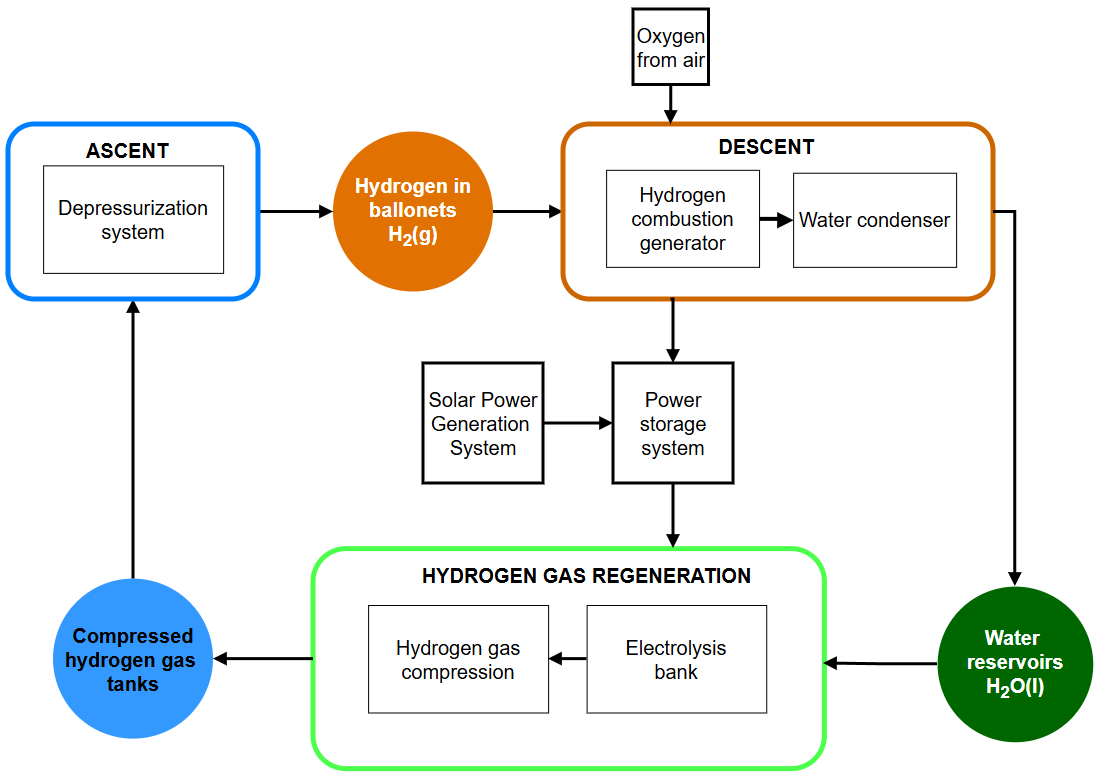
\includegraphics[width=\linewidth]{DIAGRAMA_CICLO.png}
\caption{Regenerative H\textsubscript{2} cycle for stabilization after payload release. The blue and orange blocks represent the ascent and descent actuators respectively, both acting on the central state of the system: the H\textsubscript{2} in the ballonets. O\textsubscript{2} is extracted from the surrounding atmosphere, constituting the only external flow in the cycle. Solar regeneration extends operational autonomy but does not participate in the active maneuver.}
\label{fig:ciclo}
\end{figure}

\subsubsection{Ascent Phase}
H\textsubscript{2} stored at high pressure (350~bar) is decompressed into the ballonets through the distribution manifold. This inflow increases the displaced volume and, consequently, the net aerostatic thrust governed by Archimedes' Principle.

\subsubsection{Descent Phase}
To induce altitude loss, a minimum volumetric extraction (on the order of 1~m\textsuperscript{3}) of H\textsubscript{2} is performed from the ballonets to the generator unit, generating an aerostatic thrust deficit that initiates a controlled descent. At low altitude (10--50~m above the surface), the vehicle enters a regime where aerodynamic drag stabilizes its terminal velocity. Vectorial approach and landing control is handled by the propulsors, operating in a kinematically decoupled manner from the buoyancy system.

\subsubsection{Post-Release Stabilization Phase}
Post-release stabilization constitutes the central mechanism of the proposed control scheme. Four functionally distinct stages are identified, together implementing the anticipatory transformation of the buoyancy perturbation response:

\begin{enumerate}
\item \textbf{Proactive preconditioning:} Prior to the maneuver, a fraction of H\textsubscript{2} is preemptively purged from the ballonets, reducing static thrust to mitigate the imminent force imbalance.
\item \textbf{Release:} Upon ejection of the payload (Figure~\ref{fig:liberacion}), the vehicle undergoes a step reduction in its inertial mass, inducing a net upward thrust and a transient vertical acceleration.
\item \textbf{Controlled combustion:} The feedback control loop activates the generator unit to oxidize H\textsubscript{2} at a calculated rate that compensates for the aerostatic perturbation. The reference stoichiometric reaction is:
\begin{equation}
\mathrm{H_2(g) + \tfrac{1}{2}\,O_2(g) \rightarrow H_2O(g)},\quad \Delta H = 241\,\mathrm{kJ/mol}
\label{eq:combustion}
\end{equation}
generating water vapor with mass ratio $m_{H_2O}/m_{H_2} = 9$. When atmospheric air is used as the oxidizer, N\textsubscript{2} and trace gases act as thermal diluents without participating in the reaction; this effect is captured in the effective efficiency $\eta_\mathrm{gen} = 0.30$ adopted in the analysis.
\item \textbf{Progressive condensation:} The generated vapor passes through a heat exchanger where it transitions to liquid phase, depositing in the storage tanks. The combustion-condensation cycle achieves an effective volumetric reduction of approximately 1:1300 (calculated stoichiometrically: $\rho_{H_2} \approx 0.083$~kg/m\textsuperscript{3} at ambient conditions yields ${\approx}0.75$~L of liquid water per m\textsuperscript{3} of gas) --- each m\textsuperscript{3} of gaseous H\textsubscript{2} extracted from the ballonets is consolidated into less than 1~liter of liquid water in the tanks ---. Since aerostatic thrust depends on the volume of displaced gas rather than the total mass of the vehicle, this conversion effectively reduces net thrust: the water occupies negligible volume compared to the gas it replaces, simultaneously acting as additional ballast.
\end{enumerate}

\begin{figure}[H]
\centering
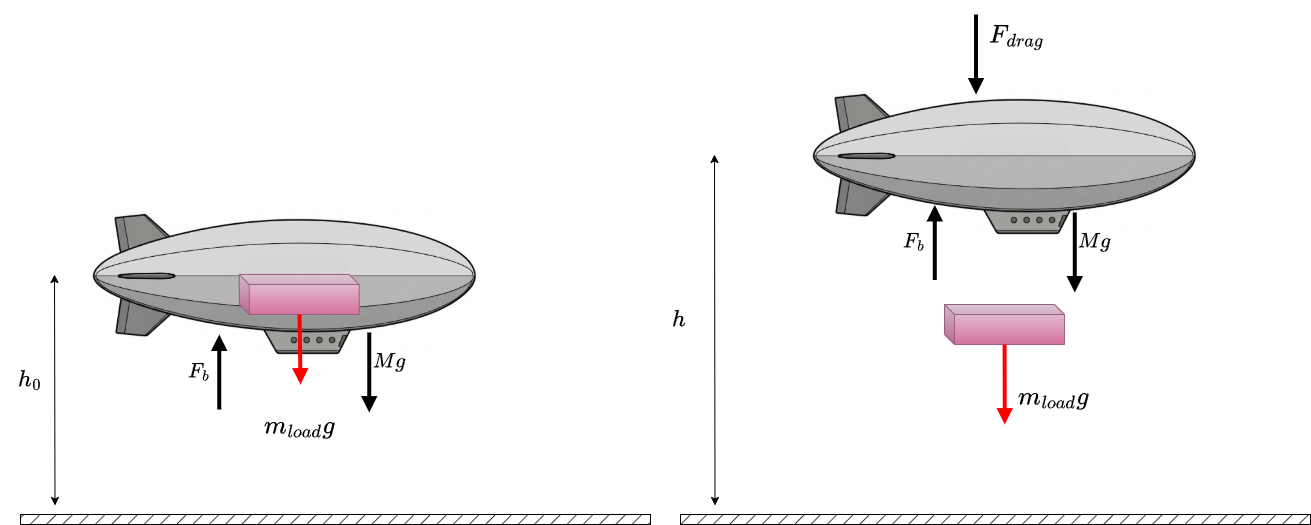
\includegraphics[width=\linewidth]{liberacion_de_carga.png}
\caption{Payload release maneuver of $m_\text{load}$ from an airship in equilibrium. The excess buoyancy activates the H\textsubscript{2} flow control. $F_\text{b}$ denotes aerostatic thrust (Archimedes), $Mg$ the total weight (structure, payload, and gas), and $F_\text{drag}$ the aerodynamic drag.}
\label{fig:liberacion}
\end{figure}

\subsubsection{Hydrogen Regeneration Phase}
The condensed water is subjected to electrolysis to dissociate and recover the consumed H\textsubscript{2}(g), which is subsequently recompressed into the main storage tanks. The energy demand of this process is supplied by two redundant sources: the photovoltaic array installed on the outer surface of the airship and the surplus electrical energy generated by the generator unit during the stabilization phase. This latter source recovers combustion energy directly as electrolysis input ($E_\text{gen} \approx 447$~kWh per delivery; Section~\ref{sec:balance}), covering approximately $22\%$ of the per-delivery electrolysis demand (${\approx}2{,}012$~kWh for $44.7$~kg H\textsubscript{2} at $45$~kWh/kg); the photovoltaic array supplies the remaining $78\%$, with self-sufficiency detailed in Section~\ref{sec:balance}.

\subsection{System Parameters and Justification}
\label{sec:params}

\begin{table}[H]
\centering
\caption{Model parameters: adopted values and operational rationale.}
\label{tab:parametros}
\renewcommand{\arraystretch}{1.3}
\resizebox{\linewidth}{!}{%
\begin{tabular}{@{} l c c @{}}
\toprule
\textbf{Parameter} & \textbf{Symbol} & \textbf{Value (Unit)} \\
\midrule
\multicolumn{3}{@{}l}{\textbf{Control and Dynamics}} \\
Damping coefficient & $\zeta$ & 1.35 \\
Proactive flow & $\dot{m}_\text{prec}$ & $-10$ kg/s \\
Anticipation time & $t_\text{anticip}$ & 2.0 s \\
Proportional gain & $K_p$ & 15 m$^3$/m \\
Derivative gain (nominal)$^{a}$ & $K_d$ & 2400 m$^3 \cdot$s/m \\
Mass control & $K_m$ & 60 kg/s/m$^3$ \\
\midrule
\multicolumn{3}{@{}l}{\textbf{Operation and Flight}} \\
Safety threshold & $|\Delta h|_\text{max}$ & 5.0 m \\
Steady-state precision & $|\Delta h|_\text{opt}$ & 1.0 m \\
Initial altitude & $h_0$ & 50 m \\
Max.\ preconditioning depth & $D_\text{lim}$ & 0.10 m \\
\midrule
\multicolumn{3}{@{}l}{\textbf{Thermodynamics and Energy}} \\
Isothermal gas temperature & $T_1$ & 288 K \\
Generator efficiency & $\eta_\text{gen}$ & 0.30 \\
Electrolysis efficiency & $\eta_\text{el}$ & 0.65 \\
Electrolysis energy demand & $E_{H_2,\text{el}}$ & 45.0 kWh/kg \\
Solar panel fraction & $f_\text{pan}$ & 0.45 \\
Solar irradiance & $r_\text{ef}$ & 2.0 kWh/m$^2$/day \\
\bottomrule
\multicolumn{3}{@{}p{\linewidth}}{$^{a}$ Nominal initial value; recalculated adaptively at each drop via Eq.~\eqref{eq:kd_app} (Appendix~B).} \\
\end{tabular}}
\end{table}

\subsubsection{Justification of Operational and Control Parameters}
To ensure the physical viability and industrial applicability of the model, the system parameters were defined based on aerospace regulations and current commercial technology limits (summarized in Table~\ref{tab:parametros}).

\textbf{Flight Dynamics and Control:} The altitude controller was tuned by imposing a strict damping coefficient of $\zeta = 1.35$. An overdamped regime is mandatory in external-load operations (such as long slings or aerial cranes) to prevent overshoots and vertical oscillations that would induce fatigue in cargo cables or the dangerous "pendulum effect" described in VERTREP (\textit{Vertical Replenishment}) manuals \cite{ref7, ref8}. The proportional-derivative controller gains ($K_p = 15$ m$^3$/m and $K_d = 2400$ m$^3 \cdot$s/m as nominal initial value) were determined to stabilize the maximum structural inertia without saturating the actuators; $K_d$ is subsequently recalculated at each drop event via Eq.~\eqref{eq:kd_app} (Appendix~B) to maintain $\zeta = 1.35$ throughout the unloading sequence. A heuristic proactive flow of $\dot{m}_\text{prec} = -10$~kg/s was also incorporated, applied 2 seconds before the release. This preconditioning extracts ${\approx}20$~kg of H\textsubscript{2} (as demonstrated numerically in Section~\ref{sec:results}), inducing an anticipated lift deficit that absorbs ${\approx}44.8\%$ of the initial upward impulse (Eq.~\eqref{eq:alpha_prec}; buoyancy reduction ${\approx}28.8\%$ plus O\textsubscript{2} ballast ${\approx}16\%$) without compromising the airship's altitude. The overdamped tuning criterion is consistent with stationkeeping control strategies reported for large high-altitude airships \cite{Schmidt2007}. Finally, a drag coefficient of $C_D = 0.5$ was adopted, representative of the vertical displacement of large-volume ellipsoidal bodies in turbulent regimes \cite{ref2, Liao2009}. \added{A proportional-derivative structure is selected over integral or state-feedback alternatives for two reasons: (i) the aerostatic system has no persistent steady-state disturbance --- the H\textsubscript{2} mass in the ballonets acts as a natural integrator, eliminating altitude error without an explicit I term; and (ii) adaptive gain scheduling handles the system nonlinearity without requiring the full state observer demanded by LQR formulations.}

\textbf{Safety and Mission Thresholds:} Simulations begin at an altitude of $h_0 = 50$~m, the typical OGE hovering altitude for aerial crane operations \cite{ref7}. Two stabilization thresholds were established: a strict safety limit of $|\Delta h| \le 5$~m, based on the maximum elongation permitted in operational slings to avoid involuntary lifting of ground equipment; and a precision threshold of $|\Delta h| \le 1$~m, required for structural coupling maneuvers. The vehicle is considered to have reached stabilization ($t_\text{stab}$) when, in addition to meeting the spatial threshold, its residual vertical velocity is below $0.05$~m/s ($0.10$~m/s for lighter airships), a safe kinematic margin for interaction with ground personnel \cite{ref7}. For the multi-release stress test, an interval of $\Delta t = 30$~s was imposed, simulating a high-intensity logistic cadence (colloquially referred to as \textit{carpet-dropping}).

\textbf{Thermodynamics and Energy Balance:} The lifting gas is modeled as isothermal at $T_1 = 288$~K (ISA sea-level standard); temperature deviations during maneuvers of $O(10)$~s are negligible relative to the convective thermal equilibration timescale of large gas envelopes. Hydrogen is supplied from tanks pressurized to 350~bar, the current standard for heavy mobility \cite{SAE2023}. The generator efficiency was set to $\eta_\text{gen} = 0.30$, a conservative lower bound for hydrogen combustion engines operating on ambient air: comprehensive reviews of H$_2$ ICEs report peak brake thermal efficiencies of 40--45\%, making 30\% a robust conservative estimate for continuous off-design operation \cite{ref9}. For the regeneration cycle, commercial PEM electrolyzers were considered with an energy demand of $45$~kWh/kg ($\eta_\text{el} \approx 0.65$), consistent with current commercial technology benchmarks \cite{ref10, Buttler2018, Falcao2020}. Solar recharging assumes a conservative mean irradiance of $r_\text{ef} = 2.0$~kWh/m$^2$/day, characteristic of the central Peruvian coast under stratocumulus cloud cover \cite{SENAMHI2003}, and a panel coverage fraction of $f_\text{pan} = 0.45$, representing the maximum effective area achievable with thin-film solar cells on the upper fuselage curvature\,\cite{Gao2024}.


\subsection{Model Assumptions and Simplifications}

\added{H$_2$ in the ballonets is modeled as an ideal gas (Eq.~\eqref{eq:gas_ideal}), valid for the pressure and temperature ranges considered. Atmospheric O\textsubscript{2} absorption during combustion is explicitly modeled as a dynamic ballast state $m_\text{water}(t)$ with stoichiometric rate $\dot{m}_\text{water} = -9\min(\dotmH,0)$; this state participates in the force balance and the equilibrium volume calculation $V_\text{eq}$ throughout the simulation. Condensation and electrolysis are treated as decoupled from the flight dynamics, with their timescales evaluated in post-processing (Section~\ref{sec:balance}). The control parameters $\dot{m}_\text{prec}$, $K_p$, $K_d$, and $K_m$ are design values selected through simulation-based tuning to satisfy the overdamped criterion ($\zeta = 1.35$; see Section~\ref{sec:params}). Each model component is grounded in a validated framework: the Newton--Euler dynamics follow Li~\&~Nahon \cite{Li2007}, validated against wind-tunnel data for airship platforms; the lifting gas is treated as isothermal at $T_1$, consistent with the short maneuver timescale ($O(10)$~s) relative to the convective equilibration of large gas envelopes; and the gain-scheduling strategy follows Moutinho et al.\ \cite{Azinheira2016}, applied and validated on real airship platforms. Internal consistency is further confirmed by the agreement between the simulated $\dotmmin$ values and the analytical scaling law (Eq.~\eqref{eq:mmin_final}): three of four platforms agree within 6\% of the analytically predicted value (Hindenburg: 2\%, Flying Whales: 3\%, Pathfinder~3: 6\%); the Zeppelin~NT achieves a value 25\% below the analytical purely-reactive bound, consistent with the greater preconditioning benefit at $\varepsilon = 0.176$.}

\subsection{Flight Dynamics Modeling}
Following the Newton--Euler vertical dynamics framework established for buoyancy-driven airships \cite{Wu2013, Li2007}, the force balance along the vertical axis is expressed as (Fig.~\ref{fig:liberacion}):

\begin{equation}
M\,\dot{v} = F_\text{b} - M\,g - F_\text{drag}
\label{eq:newton}
\end{equation}

where $M(t)$ is the total inertial mass (structure, payload, gas in the ballonets, and water ballast accumulated during combustion),
$F_\text{b}$ the aerostatic thrust (Archimedes' principle, Eq.~\eqref{eq:arquimedes}),
and $F_\text{drag}$ the aerodynamic drag (Eq.~\eqref{eq:arrastre}). Upon payload release,
$M$ undergoes a step reduction while $F_\text{b}$ remains instantaneously unchanged, as it
depends exclusively on $V_{H_2}$ --- a state variable driven solely by $\dot{m}_{H_2}$.



The aerostatic thrust (Archimedes' Principle) depends on air density, which varies exponentially with altitude, and on the volume of H\textsubscript{2}:

\begin{equation}
F_\text{b} = \rho_\text{air}(h)\,g\,V_{H_2}\, \quad
\rho_\text{air}(h) = \rho_0\,e^{-h/H_s}
\label{eq:arquimedes}
\end{equation}

The gas volume is obtained from the ideal gas law:

\begin{equation}
V_{H_2} = \frac{m_{H_2}\,R_{H_2}\,T_1}{P_\text{atm}}
\label{eq:gas_ideal}
\end{equation}

where $T_1 = 293$~K is the isothermal gas temperature (temperature deviations during $O(10)$~s maneuvers are negligible; see Section~\ref{sec:params}). The aerodynamic drag force limits the ascent velocity:

\begin{equation}
F_\text{drag} = \tfrac{1}{2}\,C_D\,A\,\rho_\text{air}(h)\,v^2\,\mathrm{sgn}(v)
\label{eq:arrastre}
\end{equation}

To simulate a multi-delivery mission, the airship mass is modeled as a time-dependent variable. The total inertial mass $M(t)$ decreases in a staircase pattern with each delivery event:

\begin{equation}
M(t) = M_\text{str} + M_\text{load}(t) + m_{H_2}(t) + m_\text{water}(t)
\end{equation}

where $m_\text{water}(t)$ is the water ballast accumulated via atmospheric O\textsubscript{2} absorption during combustion ($\dot{m}_\text{water} = -9\,\min(\dotmH,\,0)$, from the stoichiometric ratio 1:8 H\textsubscript{2}:O\textsubscript{2}), and the remaining payload $M_\text{load}(t)$ after $k(t)$ deliveries of mass $m_\text{drop}$ separated by interval $\Delta t$ is:

\begin{equation}
M_\text{load}(t) = M_\text{load}^\text{ini} - k(t) \cdot m_\text{drop}, \quad k(t) = \min\left(\lfloor t / \Delta t \rfloor,\, n\right)
\end{equation}

where $n$ is the total number of scheduled deliveries. This time-varying nature introduces a direct control challenge: the gains tuned for the initial mass become underdamped at lower masses, generating growing oscillations after consecutive deliveries. The proposed scheme addresses this through two complementary mechanisms: continuous adaptation of the derivative gain and proactive preconditioning prior to each release.

\subsubsection{Adaptive PD Controller and Preconditioning}
Purely reactive buoyancy control --- where the actuator responds only after the perturbation has been initiated --- imposes a fundamental constraint on actuator sizing. Upon payload release, the net upward perturbation $\Delta F = m_\text{load}\,g$ acts on the vehicle immediately; the available response time before the vertical displacement exceeds the safety threshold $h_\text{max}$ is bounded by $\tau_\text{ctrl} \approx \sqrt{2\,h_\text{max}\,M_\text{total}/(m_\text{load}\,g)}$ (Eq.~\eqref{eq:tau}). For the smallest evaluated platform (Zeppelin NT, $M_\text{total} \approx 6.6$~t), this window is approximately 2.6~s. A purely reactive controller must compensate the full perturbation within this interval, implying minimum flow rates of ${\approx}27$~kg/s (Eq.~\eqref{eq:mmin_final}) --- at the upper boundary of current industrial H\textsubscript{2} combustion capacity. The hybrid scheme proposed here addresses this constraint by transforming the problem structure \emph{before} the perturbation occurs, following the anticipatory feedforward principle established for suspended-load systems subject to predictable mass events \cite{Kowsari2024}.

The stabilization scheme combines a feedback Proportional-Derivative (PD) controller with a proactive preconditioning logic. The PD controller tracks a dynamic equilibrium volume $V_\text{eq}(t)$ recalculated at each mass variation. Following the gain-scheduling approach of Moutinho et al.\ \cite{Azinheira2016}, the derivative gain is adaptively tuned to maintain a constant damping coefficient $\zeta = 1.35$ throughout the unloading sequence, guaranteeing a strictly overdamped regime in accordance with VERTREP external-load operational criteria \cite{ref7, ref8}. The complete gain expressions and two-phase flow logic are provided in Appendix~B.

To mitigate the initial acceleration peak, the system incorporates an anticipatory extraction pulse. Two seconds before the scheduled release instant ($t_\text{drop}$), the system temporarily suspends the PD control and injects a constant negative flow. For the large-scale case studies presented in this work, this value is set to $\dot{m}_\text{prec} = -10$~kg/s. Extracting this flow for 2~seconds induces a proactive lift deficit sufficient to partially absorb the perturbation before release.
With atmospheric O\textsubscript{2} as oxidizer, the absorbed fraction is governed by the effective specific lift factor $L_\text{eff}$ (Eq.~\eqref{eq:cubic_prec}), which combines buoyancy loss and absorbed O\textsubscript{2} mass:
\begin{equation}
\frac{\Delta F}{\Delta F_\text{pert}} = L_\text{eff}\cdot\frac{|\dot{m}_\text{prec}|\,t_\text{prec}}{m_\text{load}} \approx 44.8\%
\label{eq:alpha_prec}
\end{equation}
for the nominal parameters of Table~\ref{tab:parametros}. The buoyancy-only contribution accounts for $(\rho_\text{air}/\rho_{H_2}) \times \ldots \approx 28.8\%$; the remaining ${\approx}16\%$ is provided by the O\textsubscript{2} mass absorbed and retained as water ballast during the 2-second preconditioning window. The anticipation time $t_\text{anticip} = 2.0$~s is selected such that the resulting preconditioning sinking depth (Eq.~\eqref{eq:cubic_prec}) satisfies $|\Delta h(t_\text{anticip})| \approx 0.027$~m for the Pathfinder~3 --- negligible relative to the post-drop safety threshold ($|\Delta h|_\text{max} = 5$~m) --- while remaining well within the operational bound $D_\text{lim} = 0.10$~m adopted for the minimax optimization (Table~\ref{tab:parametros}).

The hybrid control law with saturation is defined as:
\begin{equation}
\dot{m}_{H_2}(t) =
\begin{cases}
\dot{m}_\text{prec} & \text{if } t \in [t_\text{drop}-2\,\text{s},\; t_\text{drop}) \\
\text{sat}_{\dotmmax}\!\left(\dot{m}_\text{PD}(t)\right) & \text{otherwise}
\end{cases}
\end{equation}

This saturation at $\pm\dotmmax$ is the critical design parameter: if the hybrid scheme demands more flow than the system can provide, the vertical displacement exceeds the operational safety threshold. The proactive pulse qualitatively transforms this requirement: instead of requiring the actuator to compensate for an already-initiated upward impulse, it anticipates the perturbation by reducing net buoyancy \emph{before} the release. The PD controller then acts on a system that is already partially in descent, drastically reducing the reactive flow required. 


\subsection{Theoretical Analysis of Minimum Requirements}
\label{sec:theoretical}
From the linearized dynamics at the equilibrium point ($h_0$, $T_1$, $P_\text{atm}$) a lower bound is obtained for the minimum actuator capacity: the rate below which no control scheme can guarantee stabilization within $h_\text{max}$. Upon payload release, the net perturbation is $\Delta F = m_\text{load}\,g$. The thrust sensitivity to mass flow rate, from Eq.~\eqref{eq:gas_ideal}, is $(\rho_\text{air}/\rho_{H_2})\,g$. Without control, the available time before exceeding $h_\text{max}$ is:

\begin{equation}
\tau_\text{ctrl} \approx
\sqrt{\frac{2\,h_\text{max}\,M_\text{total}}{m_\text{load}\,g}}
\label{eq:tau}
\end{equation}

where $M_\text{total} - m_\text{load} \approx M_\text{total}$ has been applied under the
assumption $\varepsilon = m_\text{load}/M_\text{total} \ll 1$. This holds well for three
platforms ($\varepsilon \leq 0.010$, Table~\ref{tab:dirigibles}); for the Zeppelin~NT
($\varepsilon = 0.176$), the approximation introduces a ${\sim}9\%$ underestimate of
$\dotmmin$, acceptable for the purposes of this lower-bound derivation.

Imposing that the actuator compensates $\Delta F$ within $\tau_\text{ctrl}$:

\begin{equation}
\dotmmin \geq \frac{\rho_{H_2}}{\rho_\text{air}}
\sqrt{\frac{m_\text{load}^3\,g}{2\,h_\text{max}\,M_\text{total}}}
\label{eq:mmin_final}
\end{equation}

The result is counterintuitive: $\dotmmin$ \textbf{decreases} with $M_\text{total}$ — larger airships require less actuation capacity, not more. A high inertial mass implies a small perturbation index $\varepsilon = m_\text{load}/M_\text{total}$, slow post-release acceleration and more available time to respond. The parametric sweep quantifies this trend across four representative cases.

\subsection{Analytical Bound Under Hybrid Preconditioning}
\label{sec:hybrid_bound}

\added{The reactive lower bound of Section~\ref{sec:theoretical} assumes the actuator responds exclusively \emph{after} the perturbation has occurred. In the hybrid scheme, the proactive extraction pulse transforms the problem before the release: H\textsubscript{2} exits the ballonets while the vehicle simultaneously absorbs atmospheric O\textsubscript{2} for combustion, yielding a net downward force that grows linearly in time. Applying Newton's second law to this forcing and integrating twice yields a cubic displacement profile (Appendix~A):}

\begin{equation}
|\Delta h(t)| = \frac{L_\text{eff}\,g\,|\dot{m}|}{6\,M_\text{total}}\,t^3, \qquad
L_\text{eff} = \frac{\rho_\text{air}}{\rho_{H_2}} + 8
\label{eq:cubic_prec}
\end{equation}

\added{where $L_\text{eff}$ is the effective specific lift factor that accounts for both the lost buoyancy and the atmospheric O\textsubscript{2} mass absorbed during combustion ($8$~kg per kg of H\textsubscript{2} consumed, from stoichiometry). The cubic exponent arises because a constant extraction rate produces a linearly growing net force, which integrates twice to a position profile cubic in time.}

\added{Since the preconditioning and post-release stabilization phases share the same combustion hardware, the installed actuator capacity $\dotmmax$ must satisfy the peak demand of whichever phase is more intensive. The optimal distribution of the compensation burden between both phases is formulated as a minimax problem (Appendix~A):}

\begin{equation}
\dotmstar = \min_{\alpha \in [0,1]} \Bigl(\max\bigl(\dot{m}_\text{pre}(\alpha),\;\dot{m}_\text{post}(\alpha)\bigr)\Bigr)
\label{eq:minimax}
\end{equation}

\added{where $\alpha$ is the proactive compensation fraction, $\dot{m}_\text{pre}(\alpha) \propto \alpha^{3/2}$ is monotonically increasing, and $\dot{m}_\text{post}(\alpha) \propto (1-\alpha)$ is monotonically decreasing. The global minimum of the peak demand occurs at their intersection $\alpha^*$, which reduces to a depressed cubic polynomial with a unique physical root. This root is resolved in closed form via Cardano's method in the high-inertia regime ($\Delta > 0$) and Vieta's trigonometric substitution in the low-inertia regime ($\Delta \leq 0$) --- full derivations in Appendix~A. The resulting minimum required flow preserves the $M_\text{total}^{-1/2}$ scaling of Eq.~\eqref{eq:mmin_final}:}

\begin{equation}
\dotmstar \propto \frac{m_\text{load}^{3/2}}{\sqrt{M_\text{total}}}
\label{eq:mstar_scaling}
\end{equation}

\added{Figure~\ref{fig:dlim_flujo} maps $\dotmstar$ as a function of the maximum allowed preconditioning sinking depth $D_\text{lim}$ for the four evaluated platforms. For the minimax-optimal validation of Section~\ref{sec:dynval}, $D_\text{lim} = 0.10$~m is adopted as a conservative operational bound: it satisfies $D_\text{lim} \ll |\Delta h|_\text{max} = 5$~m (2\% of the safety threshold) while providing sufficient preconditioning depth for meaningful compensation. At this operational depth, the analytical minimax bound lies within 15--25\% of the numerically simulated values reported in Table~\ref{tab:minimos_actualizada}; the residual gap is attributable to aerodynamic drag and finite-mass effects not captured in the drag-free analytical model.}

\begin{figure}[H]
\centering
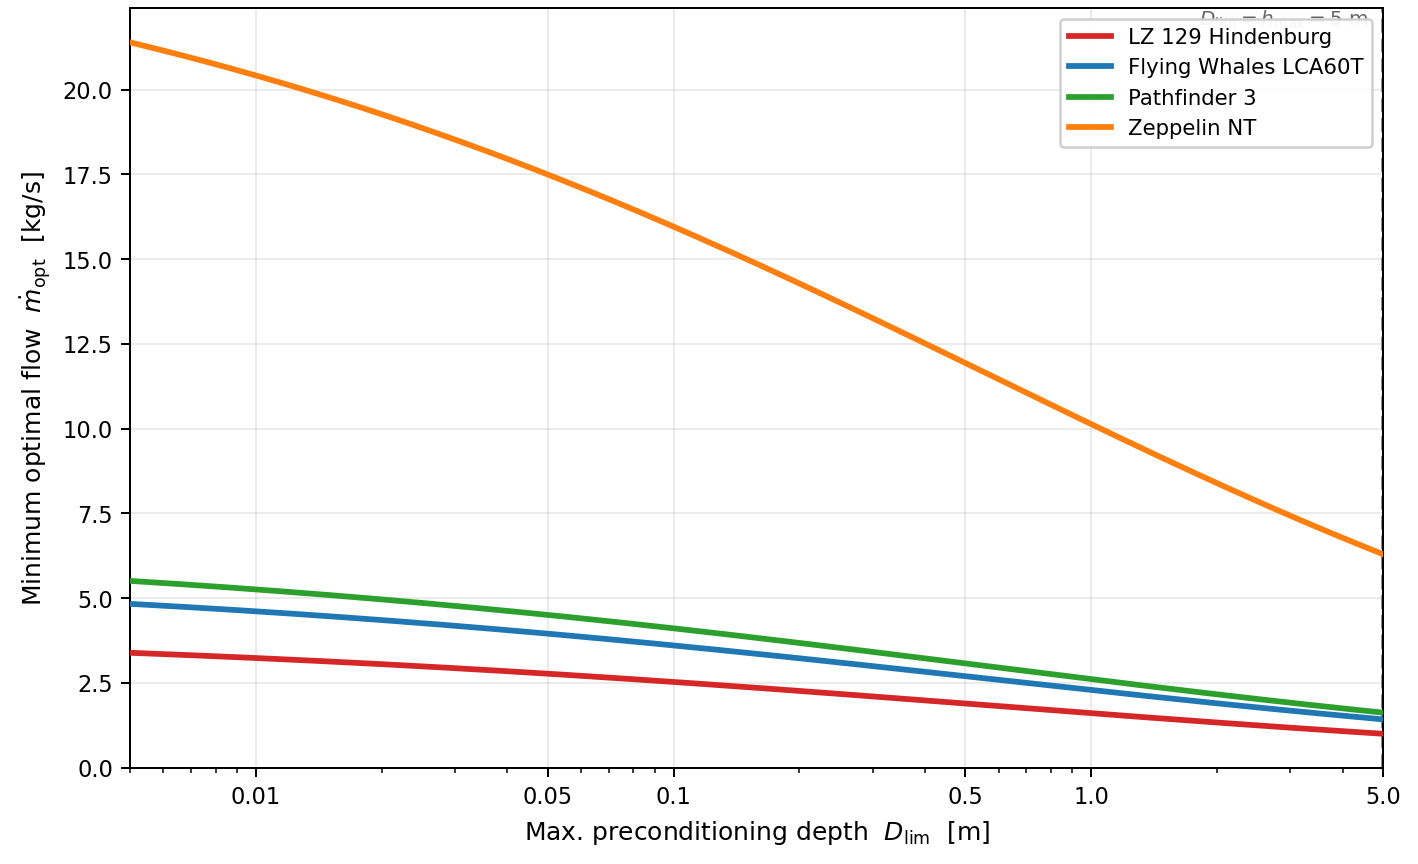
\includegraphics[width=\linewidth]{apendice_dlim_flujo_001.png}
\caption{Minimax-optimal H\textsubscript{2} combustion rate $\dotmstar$ as a function of the maximum allowed preconditioning depth $D_\text{lim}$ (Eq.~\eqref{eq:minimax}; derivations in Appendix~A). Each curve corresponds to one evaluated airship. The $M_\text{total}^{-1/2}$ scaling is directly visible: larger platforms achieve lower installed capacity requirements at every $D_\text{lim}$. The right boundary ($D_\text{lim} = 5$~m) coincides with the operational safety threshold $h_\text{max}$; the working point of the numerical simulations (Section~\ref{sec:results}) lies in the low-$D_\text{lim}$ region of each curve.}
\label{fig:dlim_flujo}
\end{figure}

%%%%%%%%%%%%%%%%%%%%%%%%%%%%%%%%%%%%%%%%%%
\section{Results}
\label{sec:results}

\subsection{Numerical Simulation and Representative Cases}
\added{The four platforms were selected to span the full range of structural masses documented for current and projected heavy-lift airships (5.6~t to 264~t), with publicly available technical specifications enabling reproducible parameter assignment. Together they represent the principal scale classes of interest for commercial heavy-lift logistics: ultralight multi-mission (Zeppelin NT), medium heavy-lift (Pathfinder~3), large-capacity (Flying Whales LCA60T), and historical reference of maximum scale (LZ~129 Hindenburg).}

Four airships are evaluated with common parameters: $m_\text{load}=1000$~kg, $h_0=50$~m (typical OGE hovering altitude for aerial crane operations \cite{ref7}) and $r_\text{ef}=2.0$~kWh/m²/day (conservative irradiance for the average cloud cover on the Peruvian coast). $A_\text{front}$ corresponds to the elliptical projection of the airship body on the horizontal plane, the reference area for drag in vertical motion. $M_\text{str}$ includes structure, systems, and operational fuel load.

\begin{table}[H]
\centering
\caption{Characteristics of the evaluated airships.}
\label{tab:dirigibles}
\renewcommand{\arraystretch}{1.2}
\setlength{\tabcolsep}{4pt}
\begin{tabular}{@{} l r r r c @{}}
\toprule
\textbf{Airship} & \makecell{$A_\text{front}$\\(m²)} & \makecell{$M_\text{str}$\\(kg)} & \makecell{$A_\text{total}$\\(m²)} & $\varepsilon$ \\
\midrule
LZ 129 Hindenburg \cite{ref2}    &  7{,}950 & 263{,}600 & 24{,}000 & 0.004 \\
Pathfinder 3$^{a}$               &  4{,}390 &  99{,}000 & 13{,}000 & 0.010 \\
Flying Whales LCA60T \cite{ref5} &  7{,}854 & 129{,}000 & 23{,}000 & 0.008 \\
Zeppelin NT \cite{ref2}          &    837   &   5{,}622 &  2{,}800 & 0.176 \\
\bottomrule
\multicolumn{5}{@{}l}{$^{a}$ Preliminary specifications from LTA Research; values are estimates.} \\
\end{tabular}
\end{table}

\subsubsection{Parametric Sweep of $\dotmmax$}
A sweep of $\dotmmax$ was performed between $0.5$ and $1000$~kg/s for each airship. For the Zeppelin NT, resolution was increased in the interval $[20, 50]$~kg/s to precisely capture the crossing of the safety thresholds. Throughout the sweep, the preconditioning pulse is bounded by the evaluated actuator capacity --- $|\dot{m}_\text{prec}| \leq \dotmmax$ --- so that at rates below $10$~kg/s the preconditioning is proportionally reduced by saturation; the reported $\dotmmin$ values are therefore conservative bounds achievable even under partial preconditioning. The maximum vertical displacement $|\Delta h|$ and stabilization time $t_\text{stab}$ were evaluated (considered reached when the residual vertical velocity falls below $0.05$--$0.10$~m/s, a safe threshold for ground personnel). \added{The peak acceleration $a_\text{max}$ is characterized analytically in Section~\ref{sec:scale}.}

\begin{figure}[H]
\centering

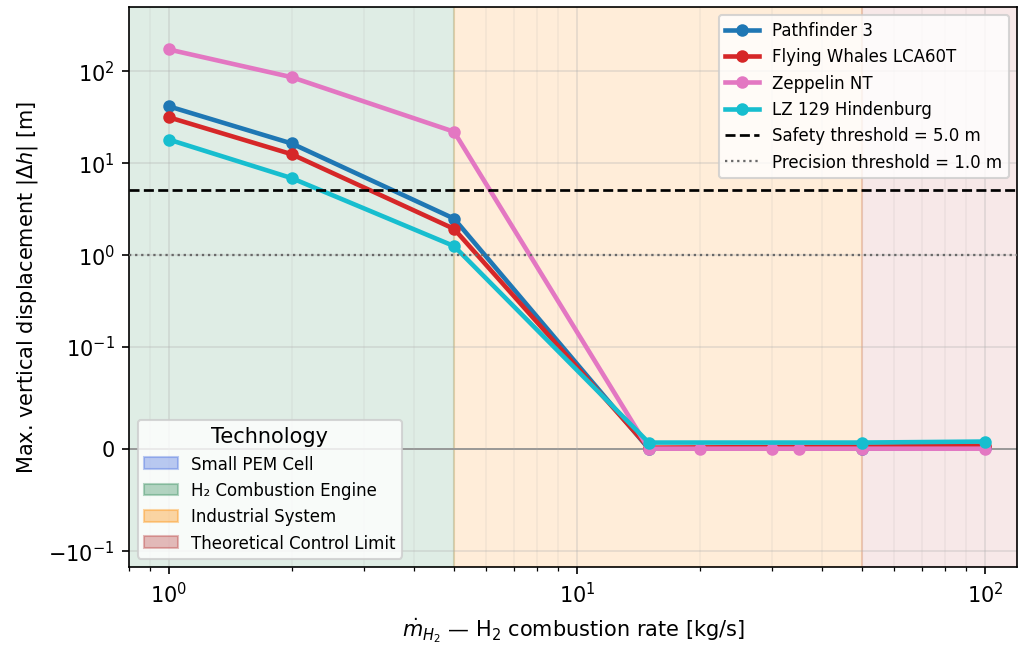
\includegraphics[width=\linewidth]{t3_o2_desplazamiento.png}
\caption{\added{Parametric sweep: maximum vertical displacement $|\Delta h|$ as a function of the H\textsubscript{2} combustion rate $\dotmH$ for each evaluated airship, accounting for O\textsubscript{2} mass absorption from atmospheric air during combustion. The safety ($5$~m, dashed) and precision ($1$~m, dotted) operational thresholds are indicated. Colored background regions classify the combustion rate by applicable technology: H\textsubscript{2} combustion engine (${\lesssim}3$~kg/s), industrial system ($3$--$20$~kg/s), and theoretical control limit (${\gtrsim}20$~kg/s). The crossing of each curve below the $5$~m line defines $\dotmmin$ for that platform; the inverse scaling with $M_\text{total}$ is directly visible (Hindenburg and Flying Whales cross at lower rates than the Zeppelin~NT). At high combustion rates, $|\Delta h|$ becomes slightly negative for large-scale platforms: the proactive preconditioning pulse initiates a controlled descent before the release event can induce any net ascent.}}
\label{fig:barrido_desp}
\end{figure}

\begin{figure}[H]
\centering

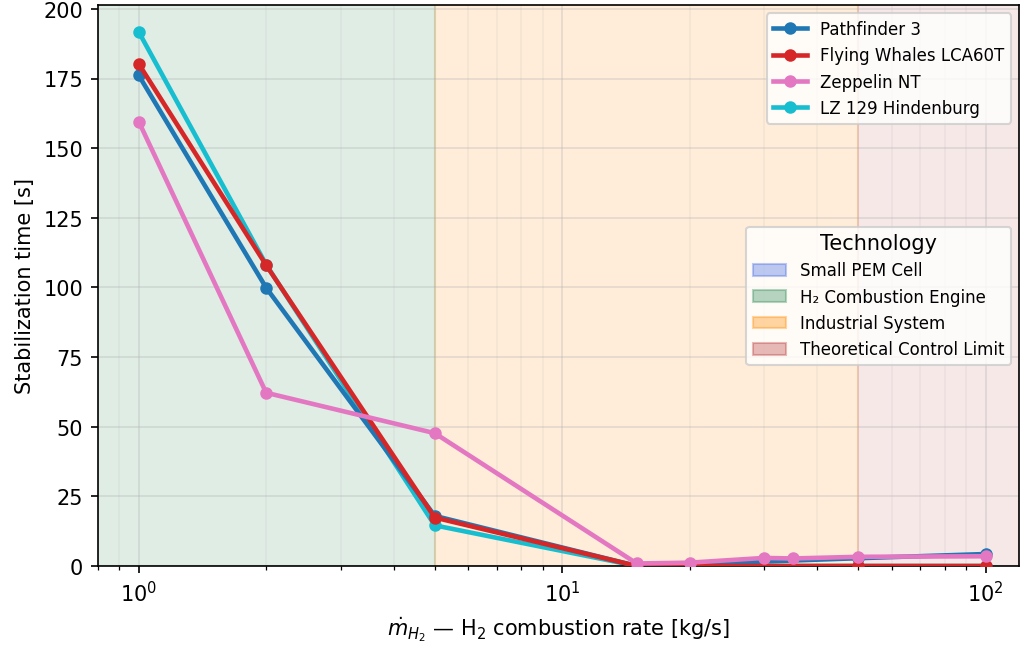
\includegraphics[width=\linewidth]{t3_o2_tiempo.png}
\caption{\added{Parametric sweep: stabilization time $t_\text{stab}$ as a function of the H\textsubscript{2} combustion rate $\dotmH$ for each evaluated airship, accounting for O\textsubscript{2} mass absorption. $t_\text{stab}$ is reached when $|\Delta h| < 1$~m and the residual vertical velocity falls below $0.05$~m/s. Technology bands follow Figure~\ref{fig:barrido_desp}. At low rates (combustion-engine range), stabilization times exceed $100$~s for all platforms. The Zeppelin~NT exhibits faster stabilization relative to large-scale platforms within the industrial-system range, consistent with its lower inertia; its $\dotmmin$ crossing at $20$~kg/s corresponds to a stabilization time of ${\approx}48$~s, reflecting the marginal nature of the safety-threshold crossing at minimum viable flow. All platforms converge below $5$~s at rates exceeding $50$~kg/s.}}
\label{fig:barrido_tiempo}
\end{figure}

Figures~\ref{fig:barrido_desp} and \ref{fig:barrido_tiempo} confirm the trends from Eq.~\eqref{eq:mmin_final}. The \textbf{Pathfinder 3} satisfies the safety threshold at $7$~kg/s and the \textbf{Flying Whales LCA60T} at $6$~kg/s, consistent with the analytical prediction of 6.6 and 5.8~kg/s respectively (within 6\% and 3\%). The \textbf{LZ~129 Hindenburg} crosses the threshold at $4$~kg/s (analytical: 4.1~kg/s, 2\% deviation). The \textbf{Zeppelin NT} crosses the $5$~m threshold at $20$~kg/s and the precision threshold at $35$~kg/s; its simulated minimum falls 25\% below the analytical purely-reactive bound (26.6~kg/s), consistent with the greater relative benefit of proactive preconditioning at $\varepsilon = 0.176$. It is notable that at extreme rates ($\geq 100$~kg/s), the displacement $|\Delta h|$ becomes slightly negative (e.g., $-0.023$~m for Pathfinder~3). This is not a numerical artifact, but evidence that the $-10$~kg/s preconditioning, not being limited by saturation of the main actuator in this phase, reduces buoyancy so aggressively that the airship initiates a controlled descent before the payload loss can induce any ascent. \added{From Figure~\ref{fig:barrido_tiempo}, the Zeppelin~NT achieves the shortest stabilization time ($3.2$~s at $\dotmopt = 35$~kg/s) despite its highest flow requirement, while the Hindenburg requires the longest ($12.4$~s), consistent with its larger inertia slowing both the perturbation and the recovery dynamics.}

\subsubsection{Minimum and Optimal Rates}
From the discrete parametric sweep, two operational thresholds are defined to classify the extraction rates $\dot{m}_{H_2,max}$:
\begin{itemize}
\item $\dotmmin$: the minimum value in the evaluated set that guarantees $|\Delta h| \leq 5$~m, in accordance with external-load operational criteria \cite{ref7,ref8} (see Section~\ref{sec:params}).
\item $\dotmopt$: the minimum value in the evaluated set that achieves $|\Delta h| \leq 1$~m, the precision threshold for structural coupling operations (see Section~\ref{sec:params}).
\end{itemize}

\begin{table}[H]
\centering
\caption{Minimum and optimal H\textsubscript{2} combustion rates for a $1000$~kg payload release. Values correspond to the discrete bounds of the parametric sweep.}
\label{tab:minimos_actualizada}
\renewcommand{\arraystretch}{1.3}
\resizebox{\linewidth}{!}{%
\begin{tabular}{@{} l cc cc c r @{}}
\toprule
& \multicolumn{2}{c}{\textbf{Safety} ($|\Delta h| \leq 5$~m)}
& \multicolumn{2}{c}{\textbf{Precision} ($|\Delta h| \leq 1$~m)}
& & \\
\cmidrule(lr){2-3}\cmidrule(lr){4-5}
\textbf{Airship}
& \makecell{$\dotmmin$\\(kg/s)}
& \makecell{$|\Delta h|$\\(m)}
& \makecell{$\dotmopt$\\(kg/s)}
& \makecell{$|\Delta h|$\\(m)}
& \makecell{$t_\text{stab}$ (s)\\(at $\dotmopt$)}
& \makecell{Analytical\\$\dotmmin$ (kg/s)\\(Eq.~\eqref{eq:mmin_final})} \\
\midrule
LZ 129 Hindenburg    & 4  & 4.697 &  8 & 0.988 & 12.4 & 4.1 \\
Pathfinder 3         & 7  & 3.286 & 20 & 0.339 &  4.4 & 6.6 \\
Flying Whales        & 6  & 3.901 & 10 & 0.958 & 10.2 & 5.8 \\
Zeppelin NT          & 20 & 3.359 & 35 & 0.650 &  3.2 & 26.6$^{a}$ \\
\bottomrule
\multicolumn{7}{@{}p{\linewidth}}{$^{a}$ Reactive analytical bound; simulated value 25\% lower due to preconditioning benefit at $\varepsilon = 0.176$.} \\
\end{tabular}}
\end{table}

From a technological standpoint, the requirements found dictate the type of subsystem needed. For the Hindenburg ($\dotmmin = 4$~kg/s) and Flying Whales LCA60T ($\dotmmin = 6$~kg/s), the requirement falls within the range of industrial H\textsubscript{2} combustion engines or large-scale premix burners. The Pathfinder~3 ($\dotmmin = 7$~kg/s) demands similar hardware at slightly higher throughput. The Zeppelin NT demands the highest flow ($\dotmmin = 20$~kg/s), requiring aeroderivative gas turbines adapted for hydrogen or high-pressure injection systems. \added{The peak post-release acceleration for each platform is bounded by $\varepsilon\,g$ and remains below $0.2\,g$ across all evaluated cases (Section~\ref{sec:scale}).}

\subsubsection{Dynamic Validation and Optimization Comparison}
\label{sec:dynval}
\added{Two controller configurations are evaluated on the Pathfinder~3 platform, corresponding to the two analytical frameworks of Sections~\ref{sec:theoretical} and \ref{sec:hybrid_bound}: a \emph{standard scheme} with hardcoded preconditioning parameters ($\dot{m}_\text{prec}{=}{-10}$~kg/s, $t_\text{anticip}{=}2$~s, $\dotmmax{=}30$~kg/s) and a \emph{minimax-optimal scheme} in which all parameters are derived analytically from Appendix~A ($\alpha^*{=}0.215$, $\dot{m}_\text{prec}{=}{-5.21}$~kg/s, $t_\text{anticip}{=}3.83$~s, $\dotmmax{=}\dotmstar{=}5.21$~kg/s).}

\paragraph{Standard scheme.}
\added{Figure~\ref{fig:sim_pf3_single} shows the single-release base case on a logarithmic time axis, which expands the resolution of the critical instants around the release at $t = 1.0$~s. The maximum vertical displacement is contained at $\Delta h \approx 0.37$~m, within the precision threshold ($1$~m). The proactive H\textsubscript{2} extraction pulse is clearly visible in the flow panel prior to release; peak acceleration remains below $0.1\,g$ throughout. A key physical mechanism is the O\textsubscript{2} mass absorption from the atmosphere: for every kilogram of H\textsubscript{2} burned, the system ingests $8$~kg of atmospheric oxygen producing $9$~kg of liquid water that acts as inertial ballast --- captured by the $L_\text{eff}$ factor in Eq.~\eqref{eq:cubic_prec}. Generated energy: ${\approx}460$~kWh per delivery cycle. A 4-drop stress test ($\Delta t = 30$~s) further confirms robustness: the adaptive gain $K_d(t)$, recalculated at each drop to maintain $\zeta = 1.35$, prevents oscillation amplification despite the step-wise reduction in inertial mass, with cumulative generated energy ${\approx}1{,}785$~kWh.}

\begin{figure}[H]
\centering
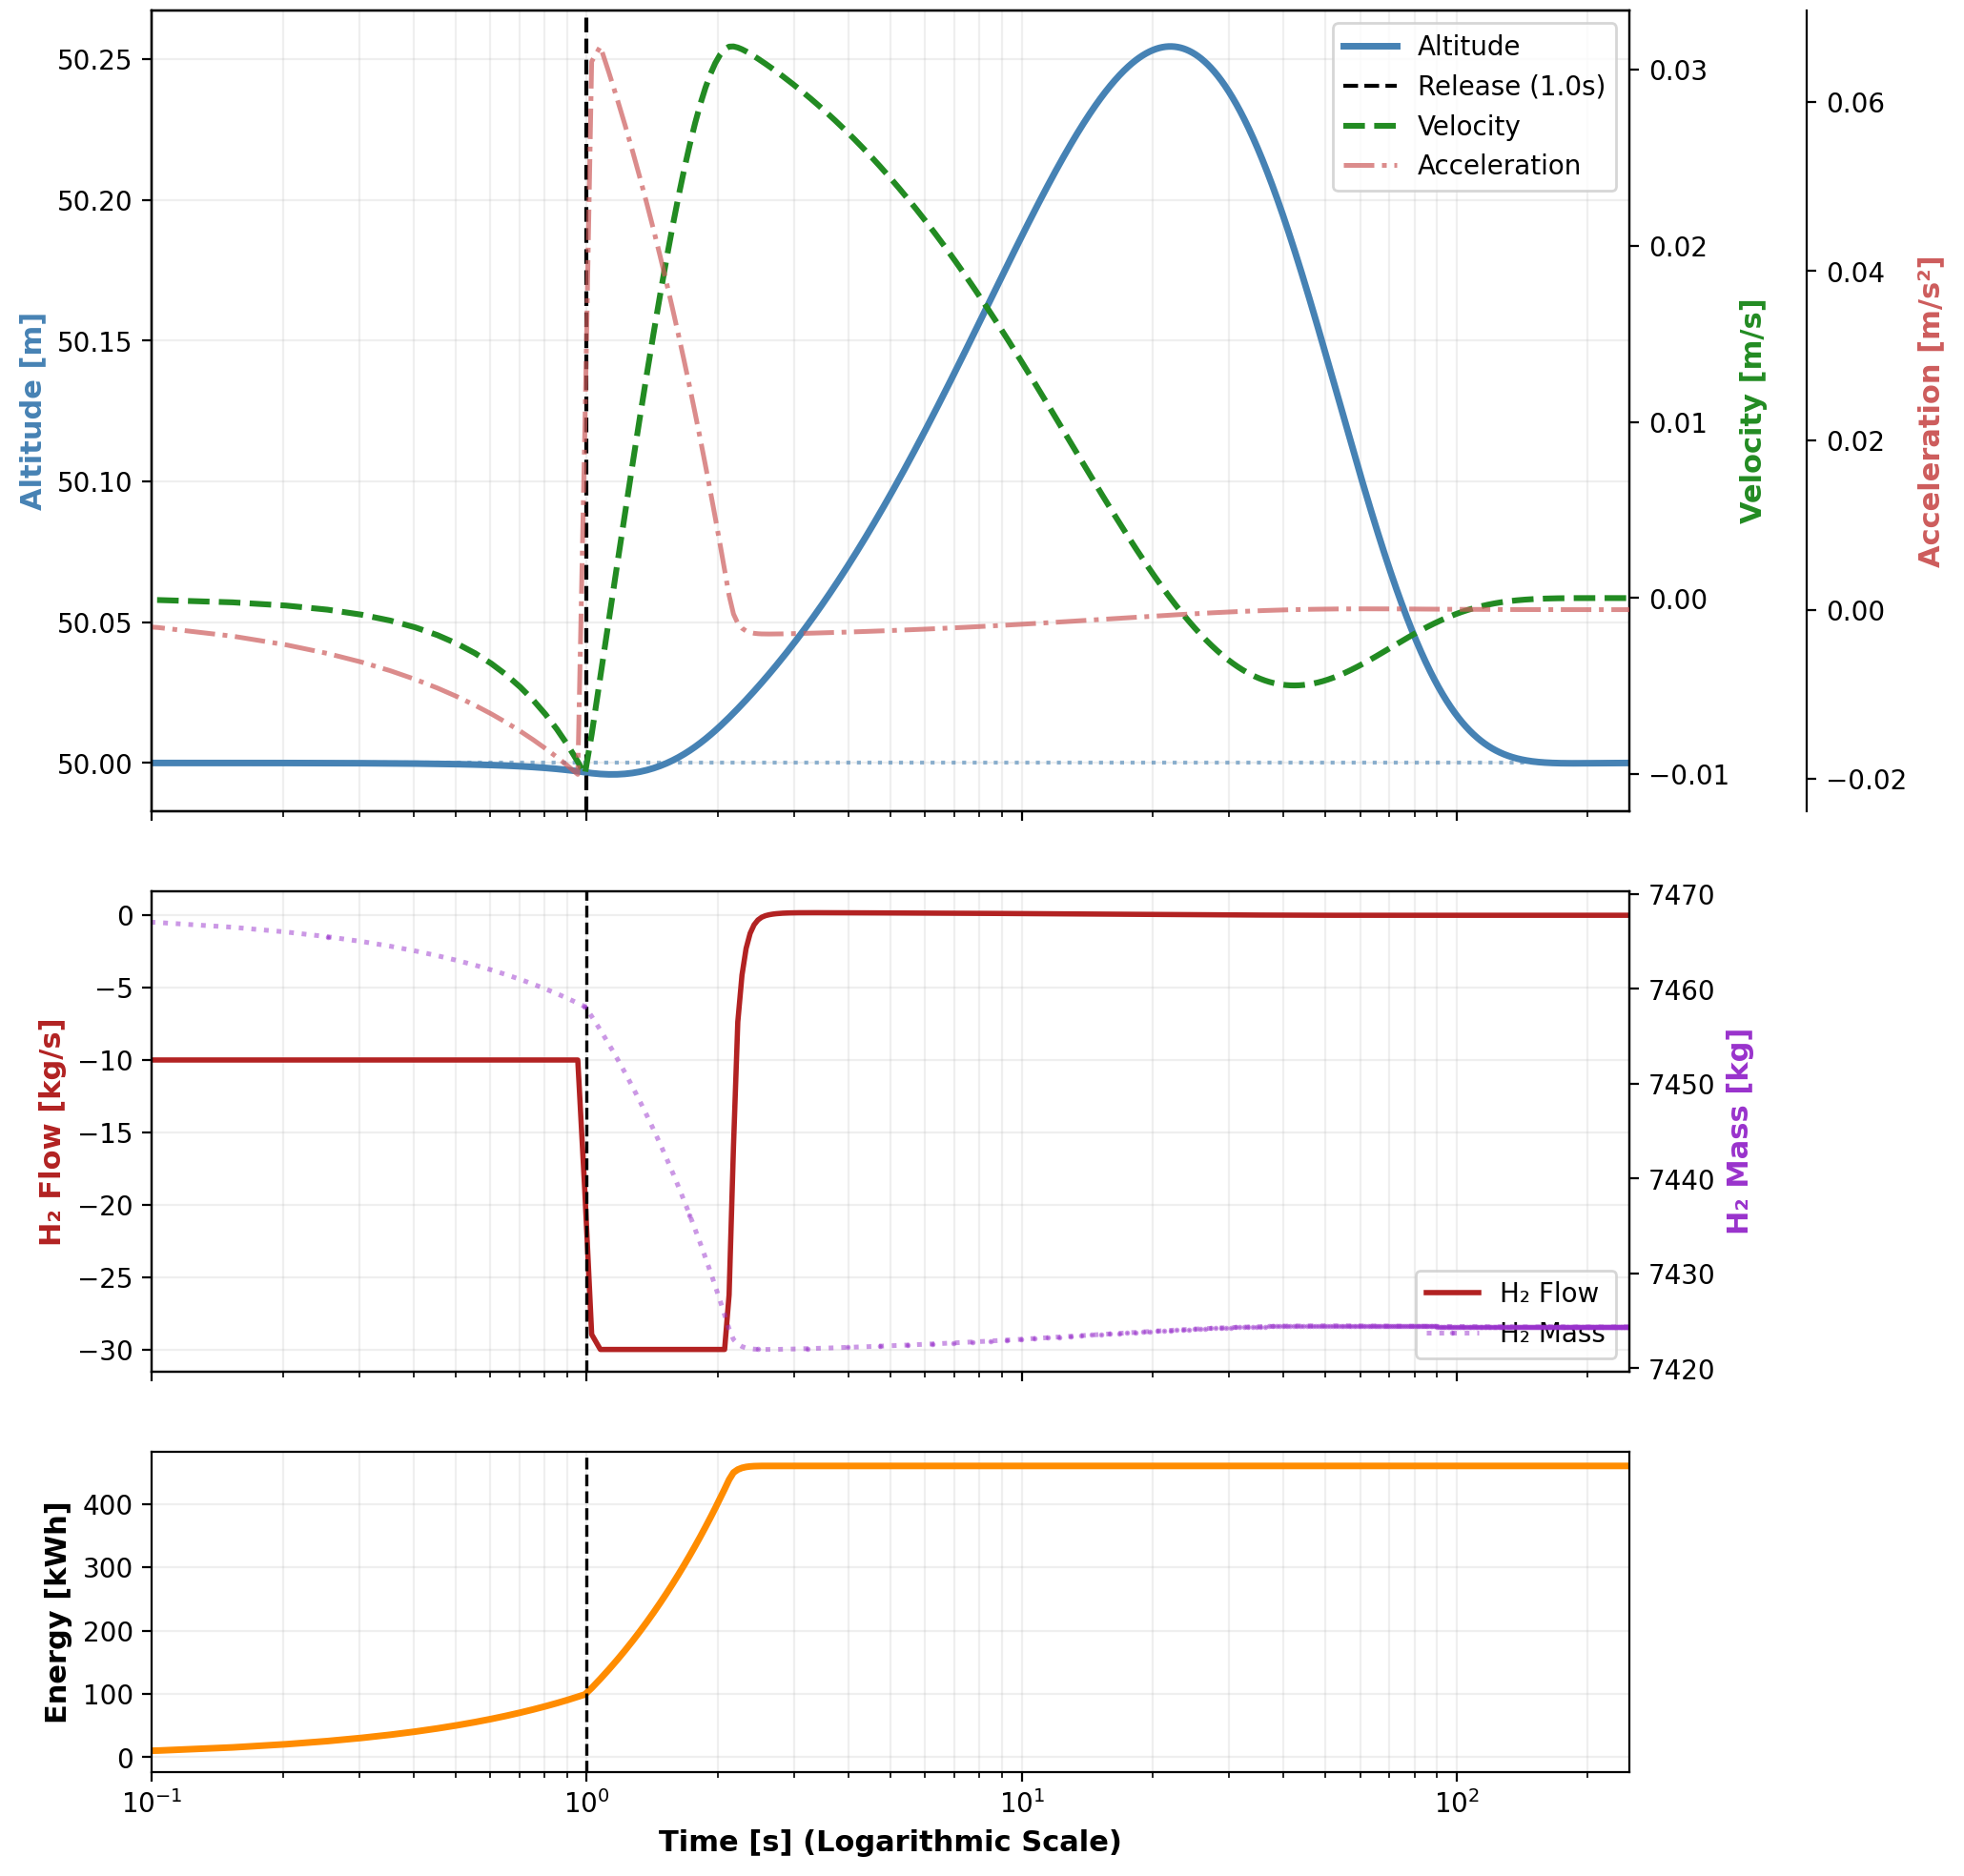
\includegraphics[width=\linewidth]{no_optimo_mision_base_final_logx.png}
\caption{Standard scheme --- Base Mission: dynamic simulation of the Pathfinder~3 ($\dotmmax{=}30$~kg/s, $\dot{m}_\text{prec}{=}{-10}$~kg/s, $t_\text{anticip}{=}2$~s) for a single 1-tonne release. Logarithmic time axis resolves the preconditioning pulse and post-release transient around $t{=}1$~s. Peak displacement $\Delta h \approx 0.37$~m satisfies the precision threshold ($1$~m).}
\label{fig:sim_pf3_single}
\end{figure}

\paragraph{Minimax-optimal scheme.}
\added{Applying the minimax formulation of Section~\ref{sec:hybrid_bound} to the Pathfinder~3, the system constant $C = 0.127$ places it in the high-inertia regime ($\Delta > 0$), yielding $\alpha^* = 0.215$ via Cardano's formula. The preconditioning parameters are recalculated analytically as $\dot{m}_\text{prec} = -5.21$~kg/s and $t_\text{anticip} = 3.83$~s, reducing the required installed actuator capacity to $\dotmstar = 5.21$~kg/s --- an $83\%$ reduction relative to the standard configuration.}

\added{Figure~\ref{fig:sim_pf3_opt_single} shows the base case with the minimax-optimal parameters on a linear time axis, resolving the extended anticipation window and the post-release recovery arc. Peak displacement reaches $\Delta h \approx 4.2$~m, within the safety threshold ($5$~m). The system converges to $(h, v) \to (h_0, 0)$ through the combined action of the overdamped PD controller ($\zeta = 1.35$) and aerodynamic drag, confirming that the minimax formulation provides the minimum installed capacity such that full state convergence is achievable --- force balance is guaranteed analytically; velocity convergence is ensured by the closed-loop PD dynamics. Generated energy: $964$~kWh, consistent with Eq.~\eqref{eq:egen} within the aerodynamic drag margin.}

\begin{figure}[H]
\centering
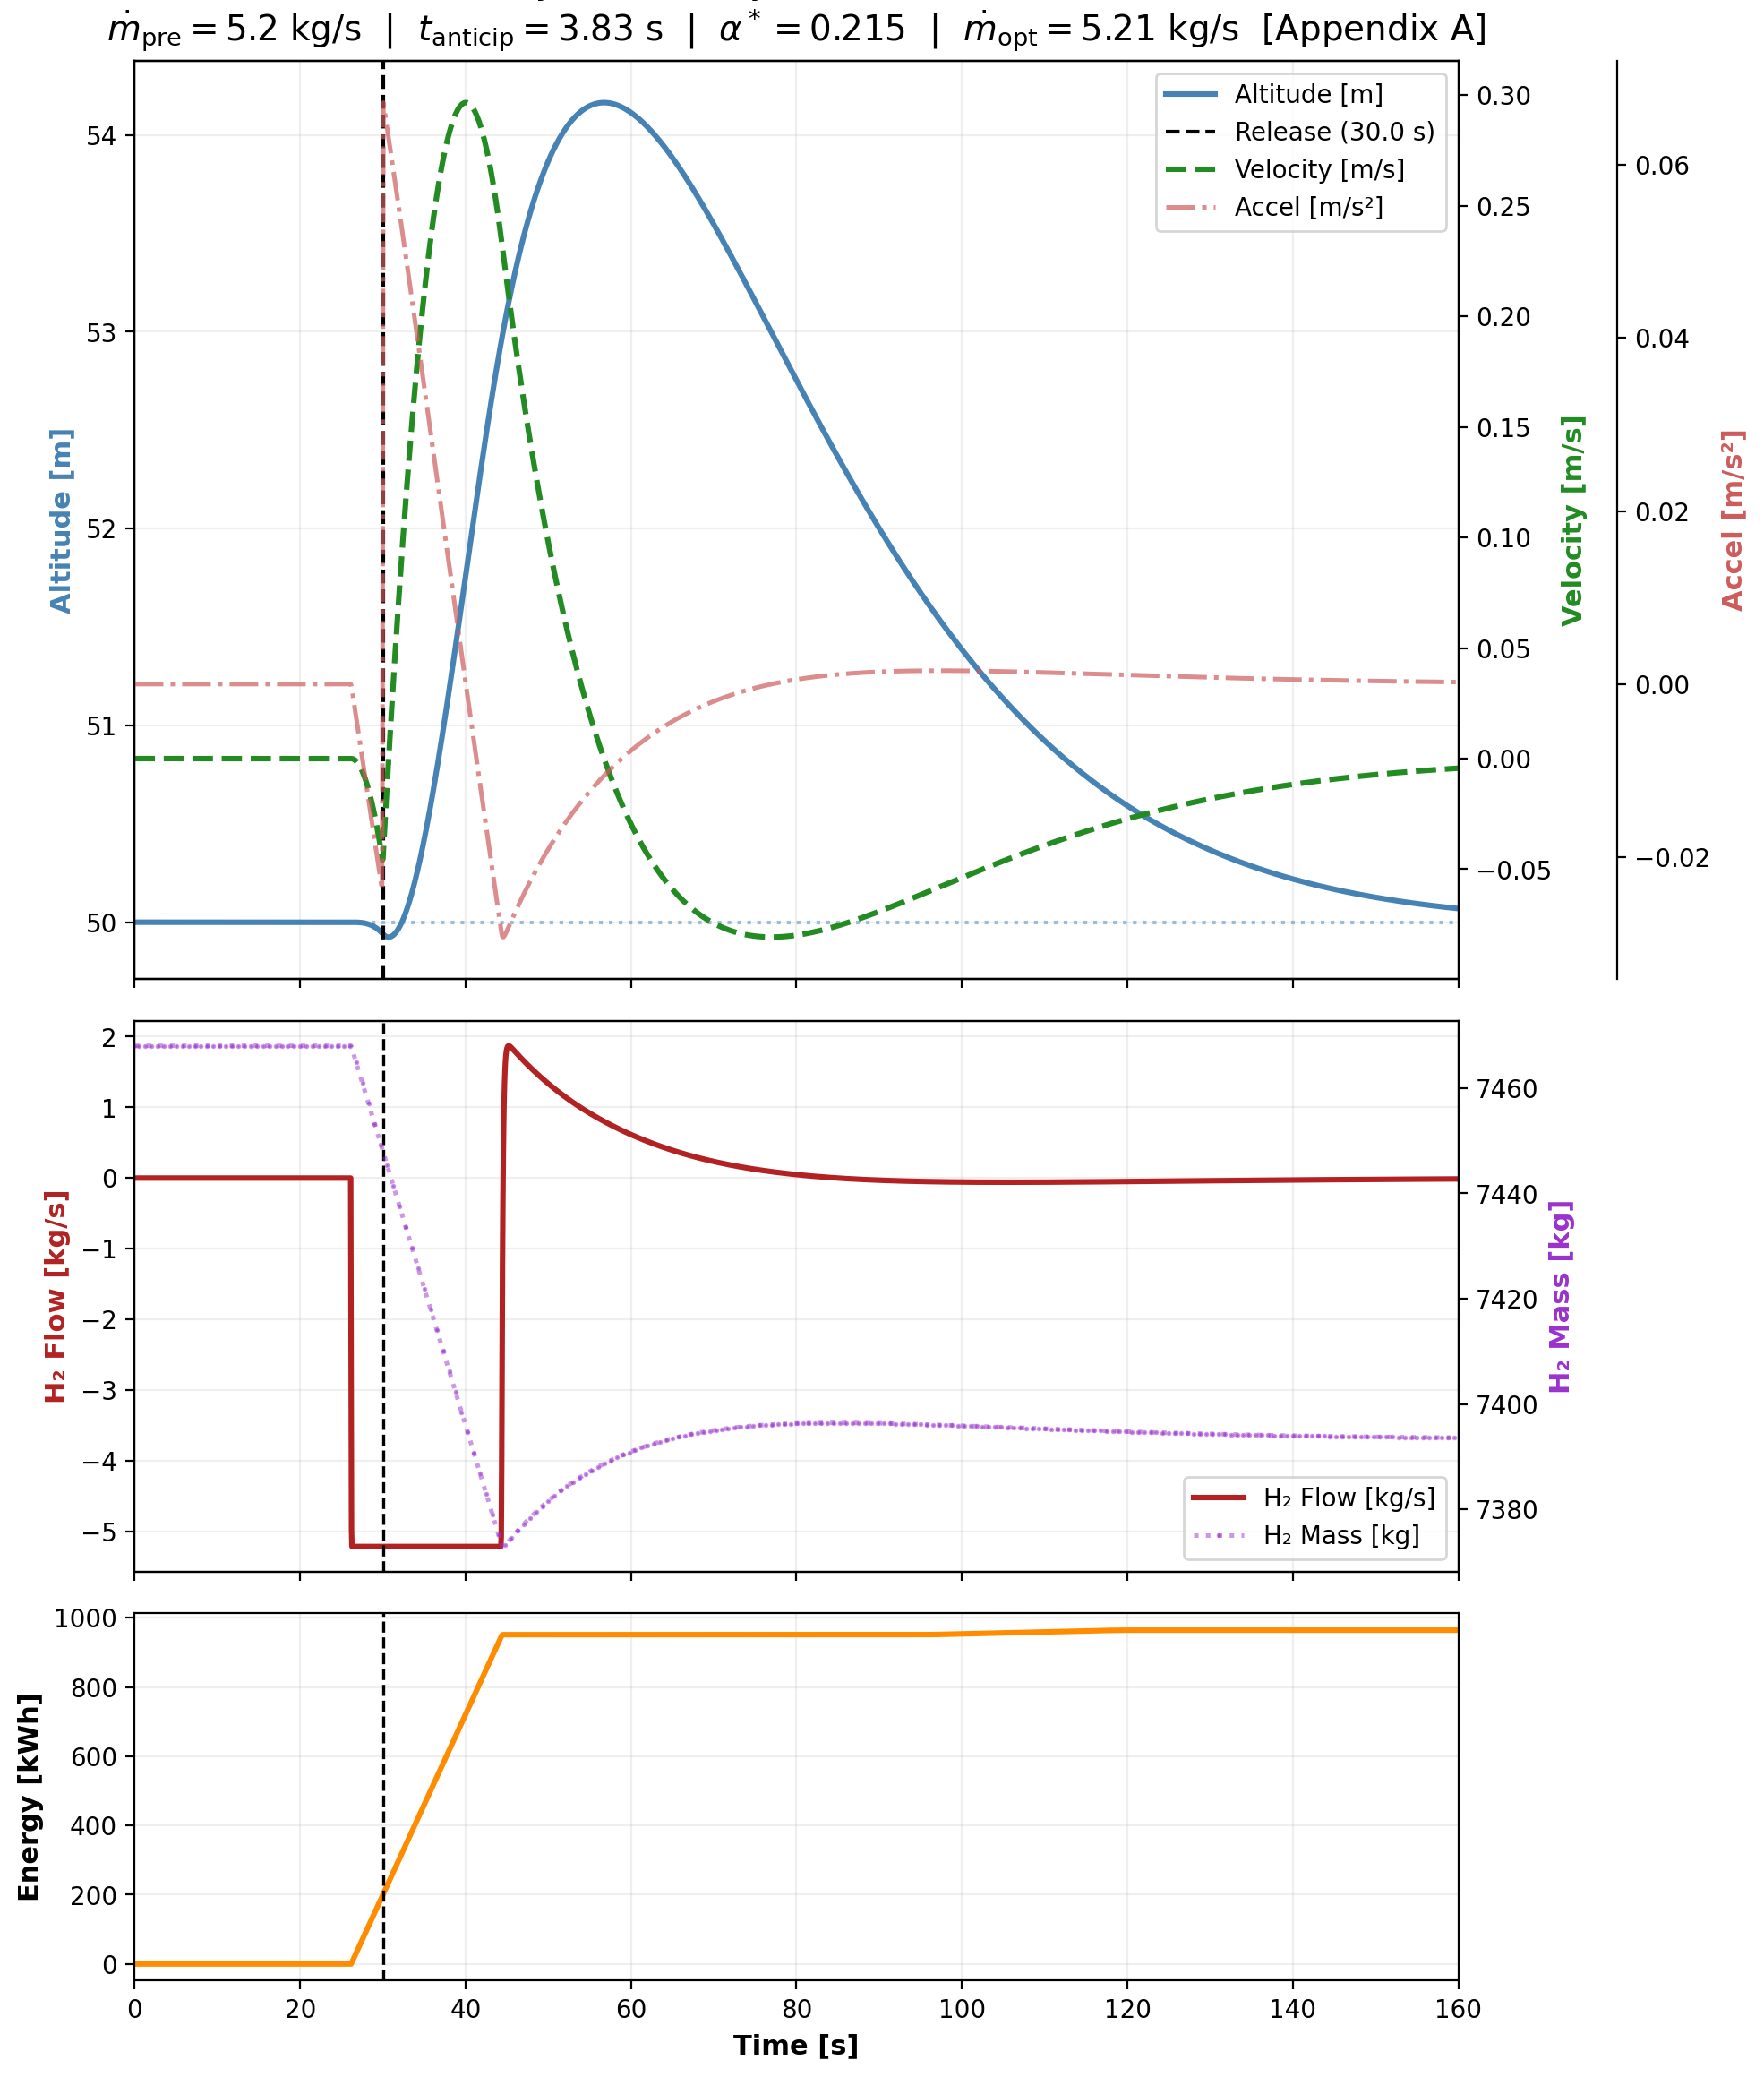
\includegraphics[width=\linewidth]{apendice_Pathfinder_3_base_001.png}
\caption{Minimax-optimal scheme --- Base Mission: dynamic simulation of the Pathfinder~3 with analytically derived parameters ($\dotmstar{=}5.21$~kg/s, $\dot{m}_\text{prec}{=}{-5.21}$~kg/s, $t_\text{anticip}{=}3.83$~s, $\alpha^*{=}0.215$; Appendix~A). Linear time axis. Peak displacement $\Delta h \approx 4.2$~m satisfies the safety threshold ($5$~m). Generated energy: $964$~kWh.}
\label{fig:sim_pf3_opt_single}
\end{figure}

\added{Figure~\ref{fig:sim_pf3_opt_multi} presents the 4-drop stress test under the optimal scheme. Both $\dot{m}_\text{prec}$ and $t_\text{anticip}$ are recalculated analytically before each drop to compensate for the decreasing vehicle mass ($\dot{m}_\text{prec}$ from $5.14$~kg/s at drop~1 to $5.21$~kg/s at drop~4; $t_\text{anticip}$ from $3.89$~s to $3.84$~s), maintaining $\alpha^*{=}0.215$ across the full unloading sequence. All four displacements remain within the safety threshold; cumulative generated energy: $3{,}586$~kWh (${\approx}897$~kWh/drop, consistent with the single-drop result within $7\%$).}

\begin{figure}[H]
\centering
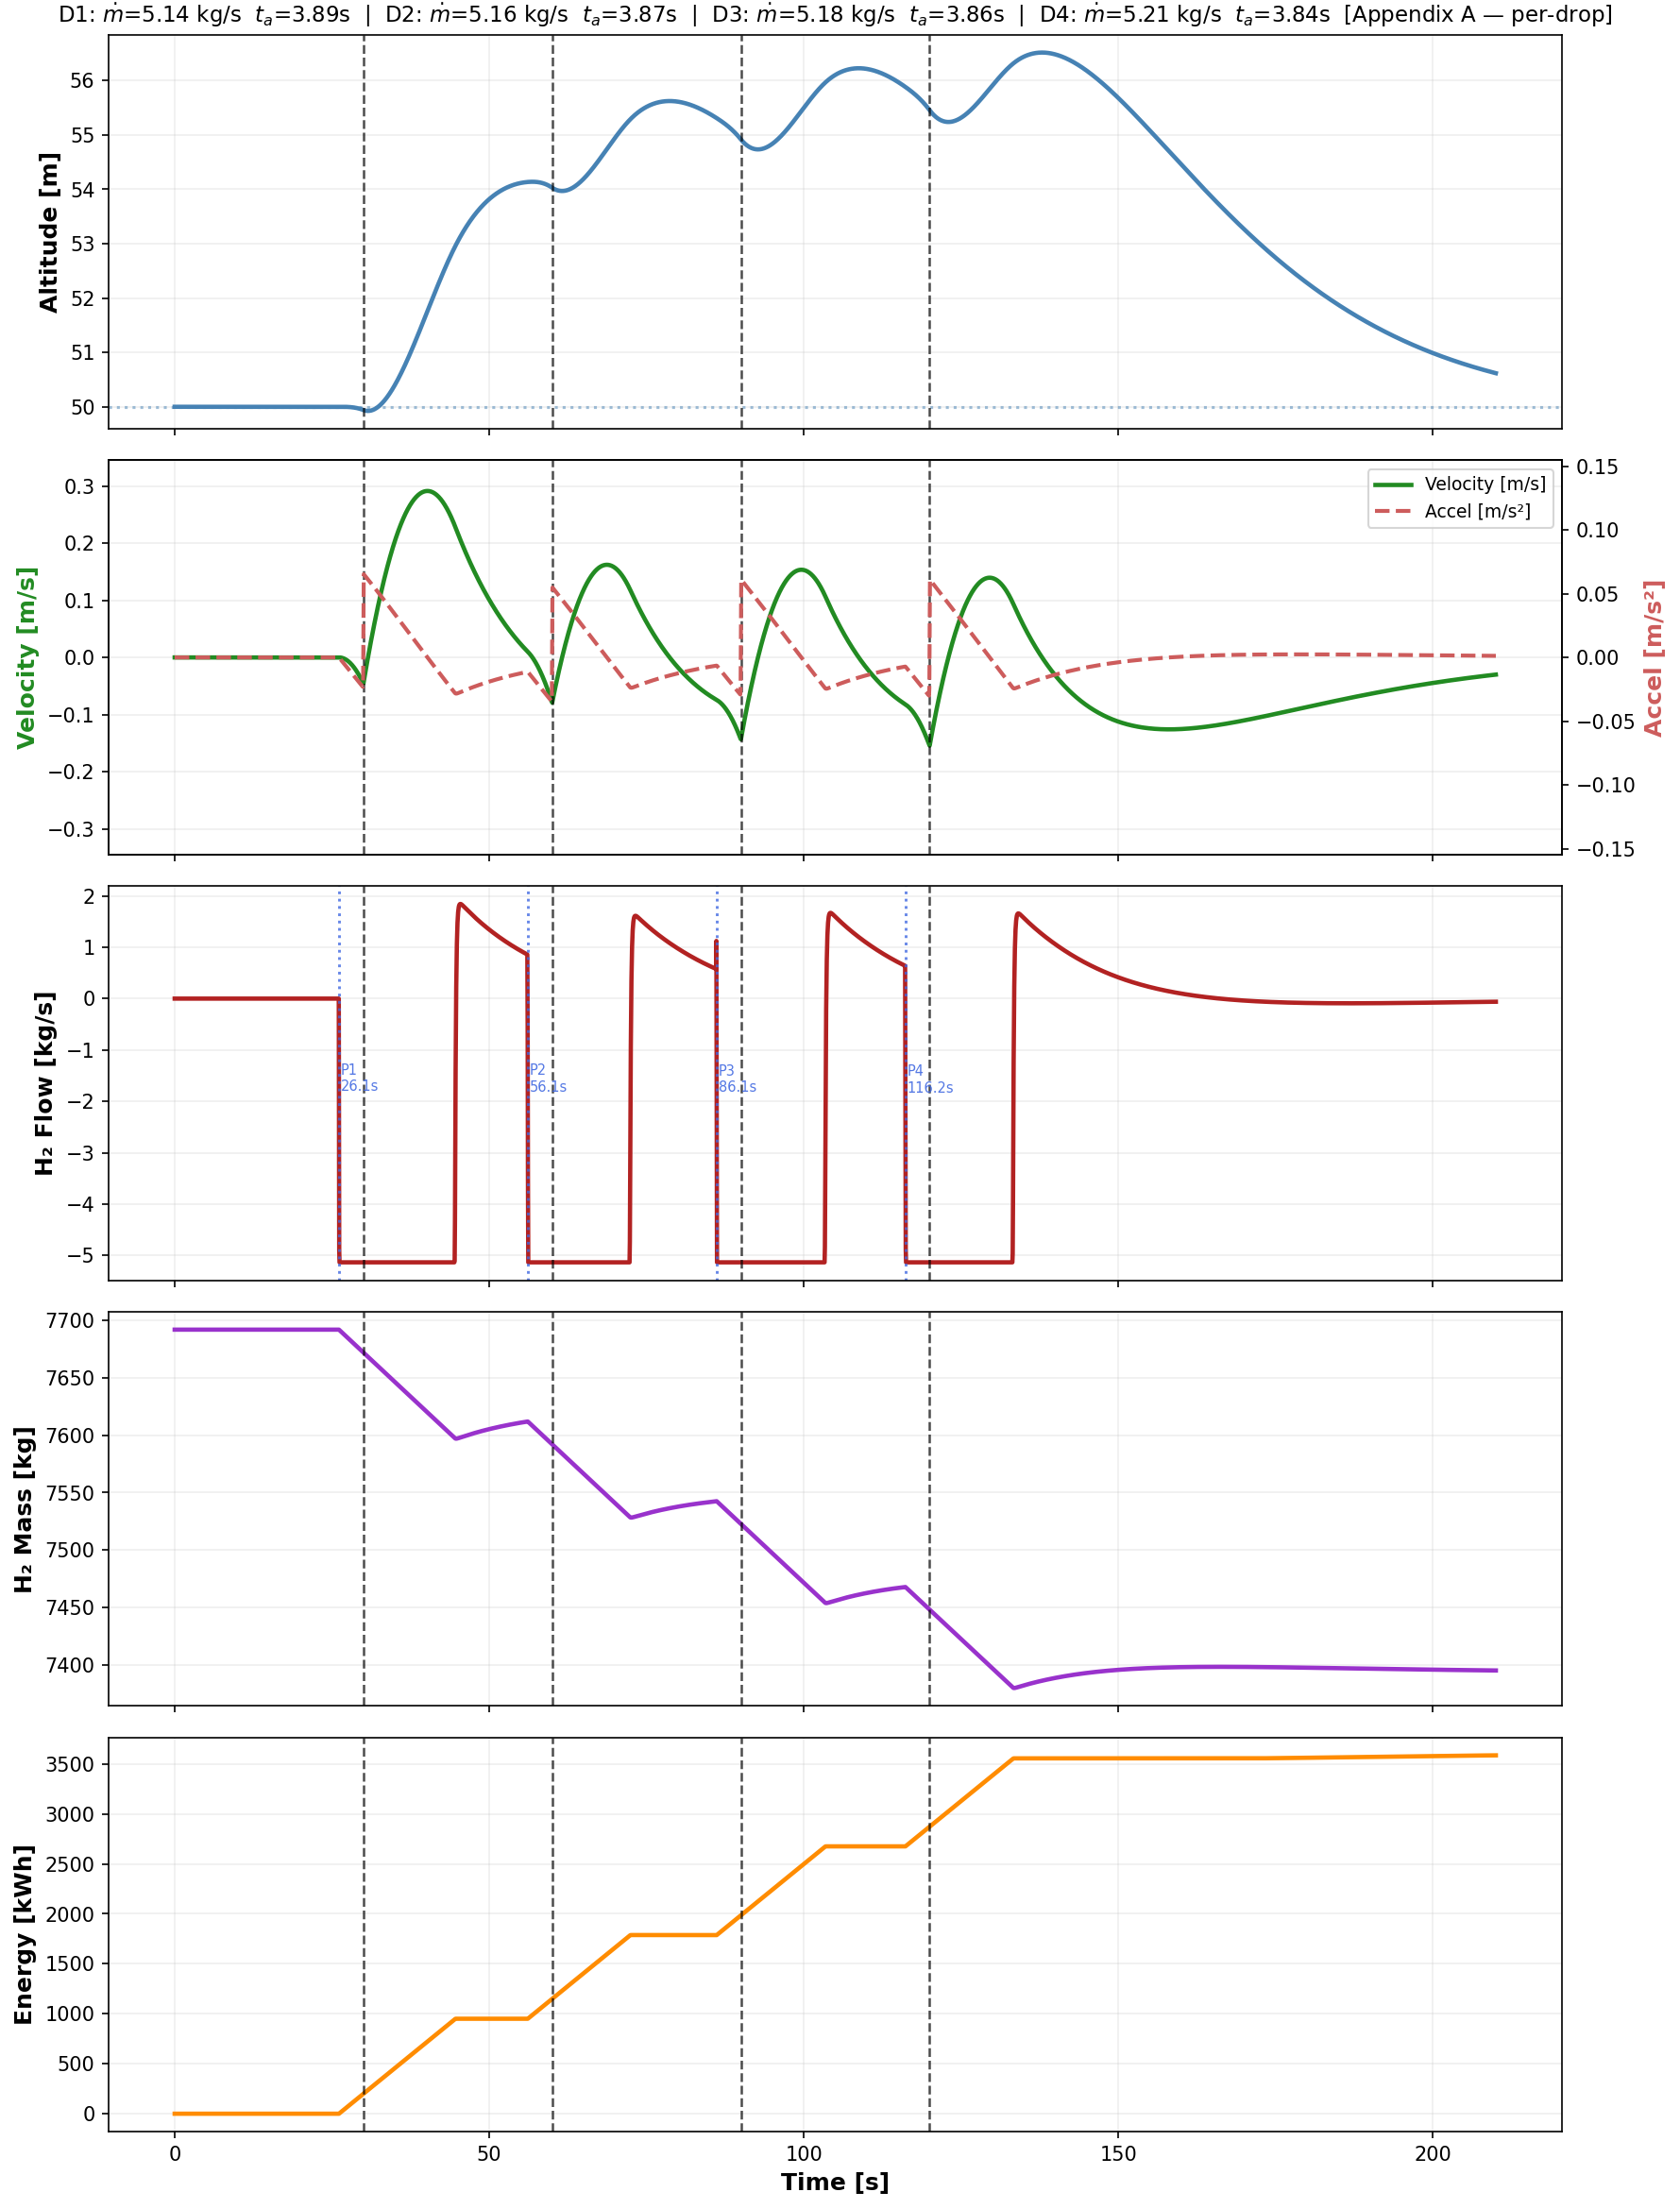
\includegraphics[width=\linewidth]{apendice_Pathfinder_3_multi4_perdrop_001.png}
\caption{Minimax-optimal scheme --- Stress Test: multi-drop mission of the Pathfinder~3 ($\dotmstar{=}5.21$~kg/s) with 4 consecutive 1-tonne releases. Optimal flow $\dot{m}_\text{prec}$ (from $5.14$ to $5.21$~kg/s) and anticipation time $t_\text{anticip}$ (from $3.89$~s to $3.84$~s) recalculated analytically before each drop to compensate for step-wise mass reduction. Cumulative generated energy: $3{,}586$~kWh.}
\label{fig:sim_pf3_opt_multi}
\end{figure}

\paragraph{Comparative summary.}
\added{Table~\ref{tab:comparison_schemes} quantifies the key differences between the two configurations. The standard scheme operates with a $6{\times}$ oversized actuator relative to the analytical minimum, achieving displacements well within the precision threshold. The minimax-optimal scheme reduces the hardware requirement to the analytical minimum at the cost of operating near the safety-threshold boundary --- the appropriate choice when minimizing installed actuator mass is the primary design constraint. In both configurations, the adaptive PD controller and the O\textsubscript{2} mass-absorption mechanism ensure full state convergence and energetic closure of the regenerative cycle.}

\begin{table}[H]
\centering
\caption{Standard vs.\ minimax-optimal control configurations for the Pathfinder~3 (single 1-tonne release).}
\label{tab:comparison_schemes}
\renewcommand{\arraystretch}{1.3}
\begin{tabular}{@{} l c c @{}}
\toprule
\textbf{Parameter} & \textbf{Standard} & \textbf{Minimax-optimal} \\
\midrule
$\dotmmax$ (kg/s)                      & 30      & 5.21 \\
$\dot{m}_\text{prec}$ (kg/s)           & $-10$   & $-5.21$ \\
$t_\text{anticip}$ (s)                 & 2.0     & 3.83 \\
$\alpha^*$                             & N/A     & 0.215 \\
$\Delta h_\text{max}$ (m)              & 0.37    & 4.2 \\
Threshold satisfied                    & Precision (${\leq}1$~m) & Safety (${\leq}5$~m) \\
$E_\text{gen}$/drop (kWh)              & ${\approx}460$ & ${\approx}964$ \\
\bottomrule
\end{tabular}
\end{table}

\subsection{Energy Balance and Auxiliary Subsystems}
\label{sec:balance}

\subsubsection{Condensation and General Balance}
With atmospheric O\textsubscript{2} as the oxidizer, the effective specific lift factor $L_\text{eff}$ (Eq.~\eqref{eq:cubic_prec}) governs both the preconditioning dynamics and the descent-phase H\textsubscript{2} consumption. Each kilogram of H\textsubscript{2} burned creates $L_\text{eff}\,g$ of net downward force through the combined effect of buoyancy loss and atmospheric O\textsubscript{2} mass absorption, so the H\textsubscript{2} required during the descent stabilization phase is:

\begin{equation}
m_{H_2,\text{desc}} = \frac{m_\text{load}}{L_\text{eff}} = \frac{m_\text{load}}{\rho_\text{air}/\rho_{H_2} + 8} \approx 44.7\,\text{kg}
\label{eq:mh2comb}
\end{equation}

This produces $m_{H_2O,\text{desc}} = 9 \times 44.7 \approx 402$~kg of water vapor in the critical condensation window. The time to recover it as liquid ballast is:

\begin{equation}
t_\text{cond} = \frac{m_{H_2O,\text{desc}}\cdot L_v}{Q_\text{cond}}, \quad L_v = 2257\,\text{kJ/kg}
\label{eq:tcond}
\end{equation}

From Eq.~\eqref{eq:tcond}, setting $t_\text{max}=10$~min as the operational cadence limit, the minimum condenser power is $Q_\text{cond,min} \approx 1{,}512$~kW (Fig.~\ref{fig:cond}).
The descent-phase stabilization acts as a secondary energy source. With $\eta_\text{gen} = 0.30$ \cite{ref9}:

\begin{equation}
E_\text{gen,desc} = m_{H_2,\text{desc}}\cdot\mathrm{PCI}_{H_2}\cdot\eta_\text{gen} \approx 447\,\text{kWh}
\label{eq:egen}
\end{equation}

This descent-phase energy recovery, ${\approx}447$~kWh per delivery, is consistent with the dynamic validation results of Section~\ref{sec:dynval} ($460$--$964$~kWh; the range reflects differing preconditioning depths and actuator capacities across the two validated configurations).

\begin{figure}[H]
\centering
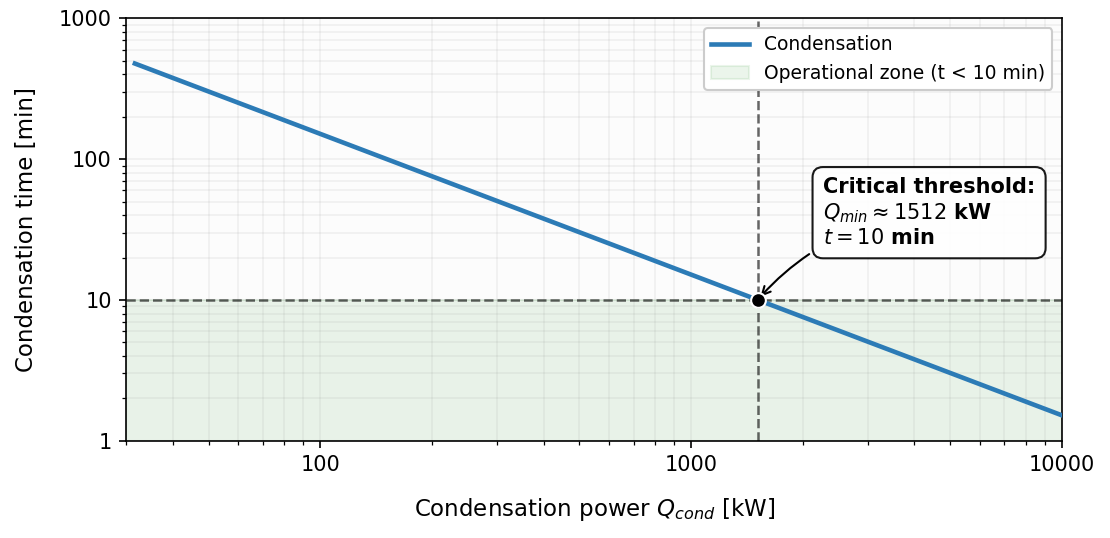
\includegraphics[width=\linewidth]{grafica_condensacion_final.png}
\caption{Condensation time vs.\ $Q_\text{cond}$ for the descent-phase water output ($m_{H_2O,\text{desc}} \approx 402$~kg, O\textsubscript{2}-corrected). The $Q_\text{cond,min} \approx 1{,}512$~kW threshold corresponds to a 10~min recovery window for the descent-phase water load.}
\label{fig:cond}
\end{figure}

This energy surplus constitutes a direct input for the electrolysis bank, optimizing the overall fuel recovery balance detailed in the following section.



%%%%%%%%%%%%%%%%%%%%%%%%%%%%%%%%%%%%%%%%%%
\section{Discussion}

\subsection{Solar Regeneration and Operational Autonomy}
Solar energy management and onboard hydrogen regeneration have been studied as autonomy-extending mechanisms in stratospheric airship platforms \cite{Zhang2019, Sun2024}. Building on this approach, the capacity to recover consumed hydrogen is modeled as a function of the available daily irradiance and the useful surface area of the vehicle. Daily regeneration is calculated using:

\begin{equation}
\dot{m}_{H_2,\text{reg}} = \frac{r_\text{ef}\cdot f_\text{pan}\cdot A_\text{total}\cdot\eta_\text{el}}{E_{H_2,\text{el}}}
\label{eq:regen}
\end{equation}

adopting as design parameters $f_\text{pan} = 0.45$ (maximum effective area assuming thin-film solar cells on the upper curvature), $\eta_\text{el} = 0.65$ and an electrolysis energy demand of $E_{H_2,\text{el}} = 45$~kWh/kg (standard values for commercial PEM cells \cite{ref10}).


Under average irradiance conditions in Lima ($2.0$~kWh/m²/day), vehicle scale dictates the viability of the closed cycle. For a single 1-tonne release, the hydrogen demand per delivery is ${\approx}44.7$~kg (descent phase, O\textsubscript{2}-corrected; see Section~\ref{sec:balance}), which sets the electrolysis regeneration target. The \textbf{LZ 129 Hindenburg} (0.14~days, 3.4~h) and the \textbf{Flying Whales} (0.15~days, 3.6~h) stand out as the efficiency benchmarks thanks to their large surface areas ($24{,}000$ and $23{,}000\text{ m}^2$ respectively). By contrast, the \textbf{Pathfinder 3} requires 0.26 days (6.4~h), while the \textbf{Zeppelin NT} ($36$~kg/day) is penalized with a recovery cycle of approximately 29.5~hours (1.23~days), exceeding the standard 24-hour delivery cadence.

Scale effects become decisive in high-intensity mission profiles. Faced with a demand of 4 consecutive releases (${\sim}179$~kg of H\textsubscript{2}), both the \textbf{Hindenburg} (0.57~days) and the \textbf{Flying Whales} (0.60~days) maintain daily self-sufficiency. The \textbf{Pathfinder 3} narrowly exceeds its daily cadence at 1.06~days, while the \textbf{Zeppelin NT} (${\approx}4.9$~days) would greatly exceed its immediate solar conversion rate. In these cases, the limitation does not lie in flight autonomy but in the water-to-gas conversion speed; the vehicle will need to draw from its pressurized H\textsubscript{2} reserve tanks while the system progressively regenerates the stored liquid ballast. This contrast underscores that the regenerative cycle is naturally optimized in large-scale airships, where the high area-to-mass ratio favors continuous unloading logistics without depleting main reserves or depending on external supply.

\subsection{Comparison with Existing Buoyancy Control Approaches}
\added{Table~\ref{tab:comparison} positions the proposed cycle within the landscape of existing buoyancy control approaches, evaluated along three operational axes: per-cycle material loss, cycle closure, and flight demonstration status.}

\begin{table}[H]
\centering
\caption{Comparison of post-release buoyancy compensation approaches.}
\label{tab:comparison}
\renewcommand{\arraystretch}{1.2}
\resizebox{\linewidth}{!}{%
\begin{tabular}{@{} l c c c c c @{}}
\toprule
\textbf{Approach} & \makecell{\textbf{Material}\\\textbf{loss}} & \makecell{\textbf{Closed-}\\\textbf{cycle}} & \makecell{\textbf{Dynamic}\\\textbf{stab.}$^{c}$} & \makecell{\textbf{Flight}\\\textbf{demo}} & \textbf{Ref.} \\
\midrule
Passive gas venting        & Yes (H\textsubscript{2}) & No            & Yes           & Yes             & \cite{ref2} \\
Consumable ballast         & Yes (ballast)            & No            & Yes           & Yes             & \cite{ref2} \\
Sliding ballast            & No                       & Partial$^{a}$ & Partial$^{a}$ & Yes             & \cite{Lanteigne2017} \\
Inflatable vacuum chambers & No                       & Yes           & No            & No              & \cite{Barton2013} \\
Active gas transfer        & Yes (H\textsubscript{2}) & No            & Partial       & Partial         & \cite{Li2007} \\
He compression (COSH)      & No                       & Yes$^{b}$     & No$^{b}$      & Yes (prototype) & \cite{Pasternak2015} \\
H\textsubscript{2} regen.\ fuel cell & No             & Yes           & No            & No              & \cite{Sun2024} \\
\textbf{This work}         & \textbf{No}$^{d}$        & \textbf{Yes}  & \textbf{Yes}  & \textbf{No (sim.)} & --- \\
\bottomrule
\multicolumn{6}{@{}p{\linewidth}}{$^{a}$ Provides attitude control but does not address net buoyancy surplus after release.} \\
\multicolumn{6}{@{}p{\linewidth}}{$^{b}$ Closed-cycle via mechanical He compression; does not integrate with the H\textsubscript{2} energy chain; no post-release stabilization.} \\
\multicolumn{6}{@{}p{\linewidth}}{$^{c}$ Active compensation of the post-release aerostatic imbalance within the safety threshold ($|\Delta h| \leq 5$~m).} \\
\multicolumn{6}{@{}p{\linewidth}}{$^{d}$ Under ideal closed-cycle assumption.}
\end{tabular}}
\end{table}

\added{Among closed-cycle approaches, COSH relies on mechanical He compression within a separate gas infrastructure and provides no post-release dynamic stabilization; regenerative fuel cells address pressure maintenance but not the transient aerostatic imbalance following a payload release. The proposed cycle is the only approach in Table~\ref{tab:comparison} that simultaneously achieves closed-cycle operation, no per-cycle material loss (under ideal closed-cycle assumption; Table~\ref{tab:comparison}, note $d$), and active post-release stabilization within a single H\textsubscript{2} chain. Beyond the system concept, this work provides analytical tools absent from prior approaches: a closed-form scaling law for the minimum actuator capacity (Eq.~\eqref{eq:mmin_final}), a minimax formulation with exact solution via Cardano's method (Section~\ref{sec:hybrid_bound}, Appendix~A), and a parametric characterization validated across four representative platforms.}

\subsection{Scale and Sensitivity}
\label{sec:scale}
The most notable result is the inversion of scale intuition: the Hindenburg (264~t) requires the lowest rate (4~kg/s), while the Zeppelin~NT (5.6~t) is the most sensitive (20~kg/s). This paradox has a direct physical explanation: a higher total mass implies a smaller perturbation index $\varepsilon = m_\text{load}/M_\text{total}$, which in turn yields a longer available response window $\tau_\text{ctrl}$ before the safety threshold is exceeded (Eq.~\eqref{eq:tau}). The actuator therefore operates against a slower-evolving perturbation, reducing the required instantaneous flow rate. This result positions the regenerative H\textsubscript{2} cycle as intrinsically suited for next-generation heavy-lift platforms, where it is precisely the largest vehicles that benefit most.

\added{Beyond the flow rate requirement, $\varepsilon$ also governs the peak post-release acceleration: $a_\text{max} = \varepsilon\,g$, bounded by $0.176\,g$ for the Zeppelin~NT --- the most dynamically sensitive platform --- and below $0.01\,g$ for the three large-scale cases. All evaluated platforms therefore satisfy an operational comfort threshold of $0.2\,g$ without additional constraint, confirming that the perturbation is dynamically significant for buoyancy control but does not impose structural or personnel-safety hazards in any of the evaluated cases.}

\subsection{Stabilization Scope: Force Balance, State Convergence, and Fine-Attitude Control}
\label{sec:stab_scope}
\added{The minimax formulation of Section~\ref{sec:hybrid_bound} determines the minimum installed capacity $\dotmstar$ such that the aerostatic force balance is achievable within the preconditioning depth $D_\text{lim}$ --- a necessary condition for stabilization. Full state convergence, $(h, v) \to (h_0, 0)$, is a stronger requirement that the minimax alone does not guarantee analytically: it is ensured by the overdamped PD controller ($\zeta = 1.35$) acting within the capacity provided by $\dotmstar$, as confirmed numerically in Section~\ref{sec:dynval}. Once force balance is achievable, the derivative term $K_d\,v$ continuously injects corrective flow proportional to the residual velocity, driving the state to rest; aerodynamic drag provides additional passive damping that reinforces convergence monotonically.}

\added{For operations at the absolute minimum installed capacity --- where the actuator is fully saturated throughout the maneuver --- a small residual velocity may persist after the buoyancy system has exhausted its authority. In practice, this residual is handled by the fine-attitude propulsion system (vectored thrusters or differential propeller pitch) employed during standard airship approach and landing procedures \cite{ref7, ref8}. This two-layer architecture --- buoyancy system for gross perturbation attenuation, fine-attitude propulsion for terminal velocity correction --- imposes no additional hardware requirements beyond the existing propulsion system and is consistent with established operational airship protocols.}

\subsection{Condensation, O$_2$ Source and Mass Balance}
The threshold $Q_\text{cond,min}=1{,}512$~kW corresponds to the scale of medium-capacity industrial heat exchangers used in chemical processing applications. The analysis adopts atmospheric O$_2$ as the reference choice, although the system equally admits onboard tanks. As demonstrated quantitatively in Figure~\ref{fig:comparacion_o2}, atmospheric air reduces the descent-phase H$_2$ burning requirement by ${\approx}35.8\%$ relative to onboard O$_2$ (from ${\approx}69.6$~kg to $44.7$~kg per tonne). The physical mechanism is as follows: with onboard O$_2$, only the buoyancy reduction contributes to stabilization (effective factor $\rho_\text{air}/\rho_{H_2} \approx 14.4$); with atmospheric air, the stoichiometric 8~kg of O$_2$ absorbed per kg of H$_2$ adds directly to the vehicle inertial mass, yielding $L_\text{eff} = \rho_\text{air}/\rho_{H_2}+8 \approx 22.4$, consistent with the O$_2$-corrected formula of Section~\ref{sec:balance}. This supplementary inertial ballast simultaneously reduces actuator flow demand and the critical-window condensation load, constituting an additional degree of freedom for mission profile design.

\begin{figure}[H]
\centering
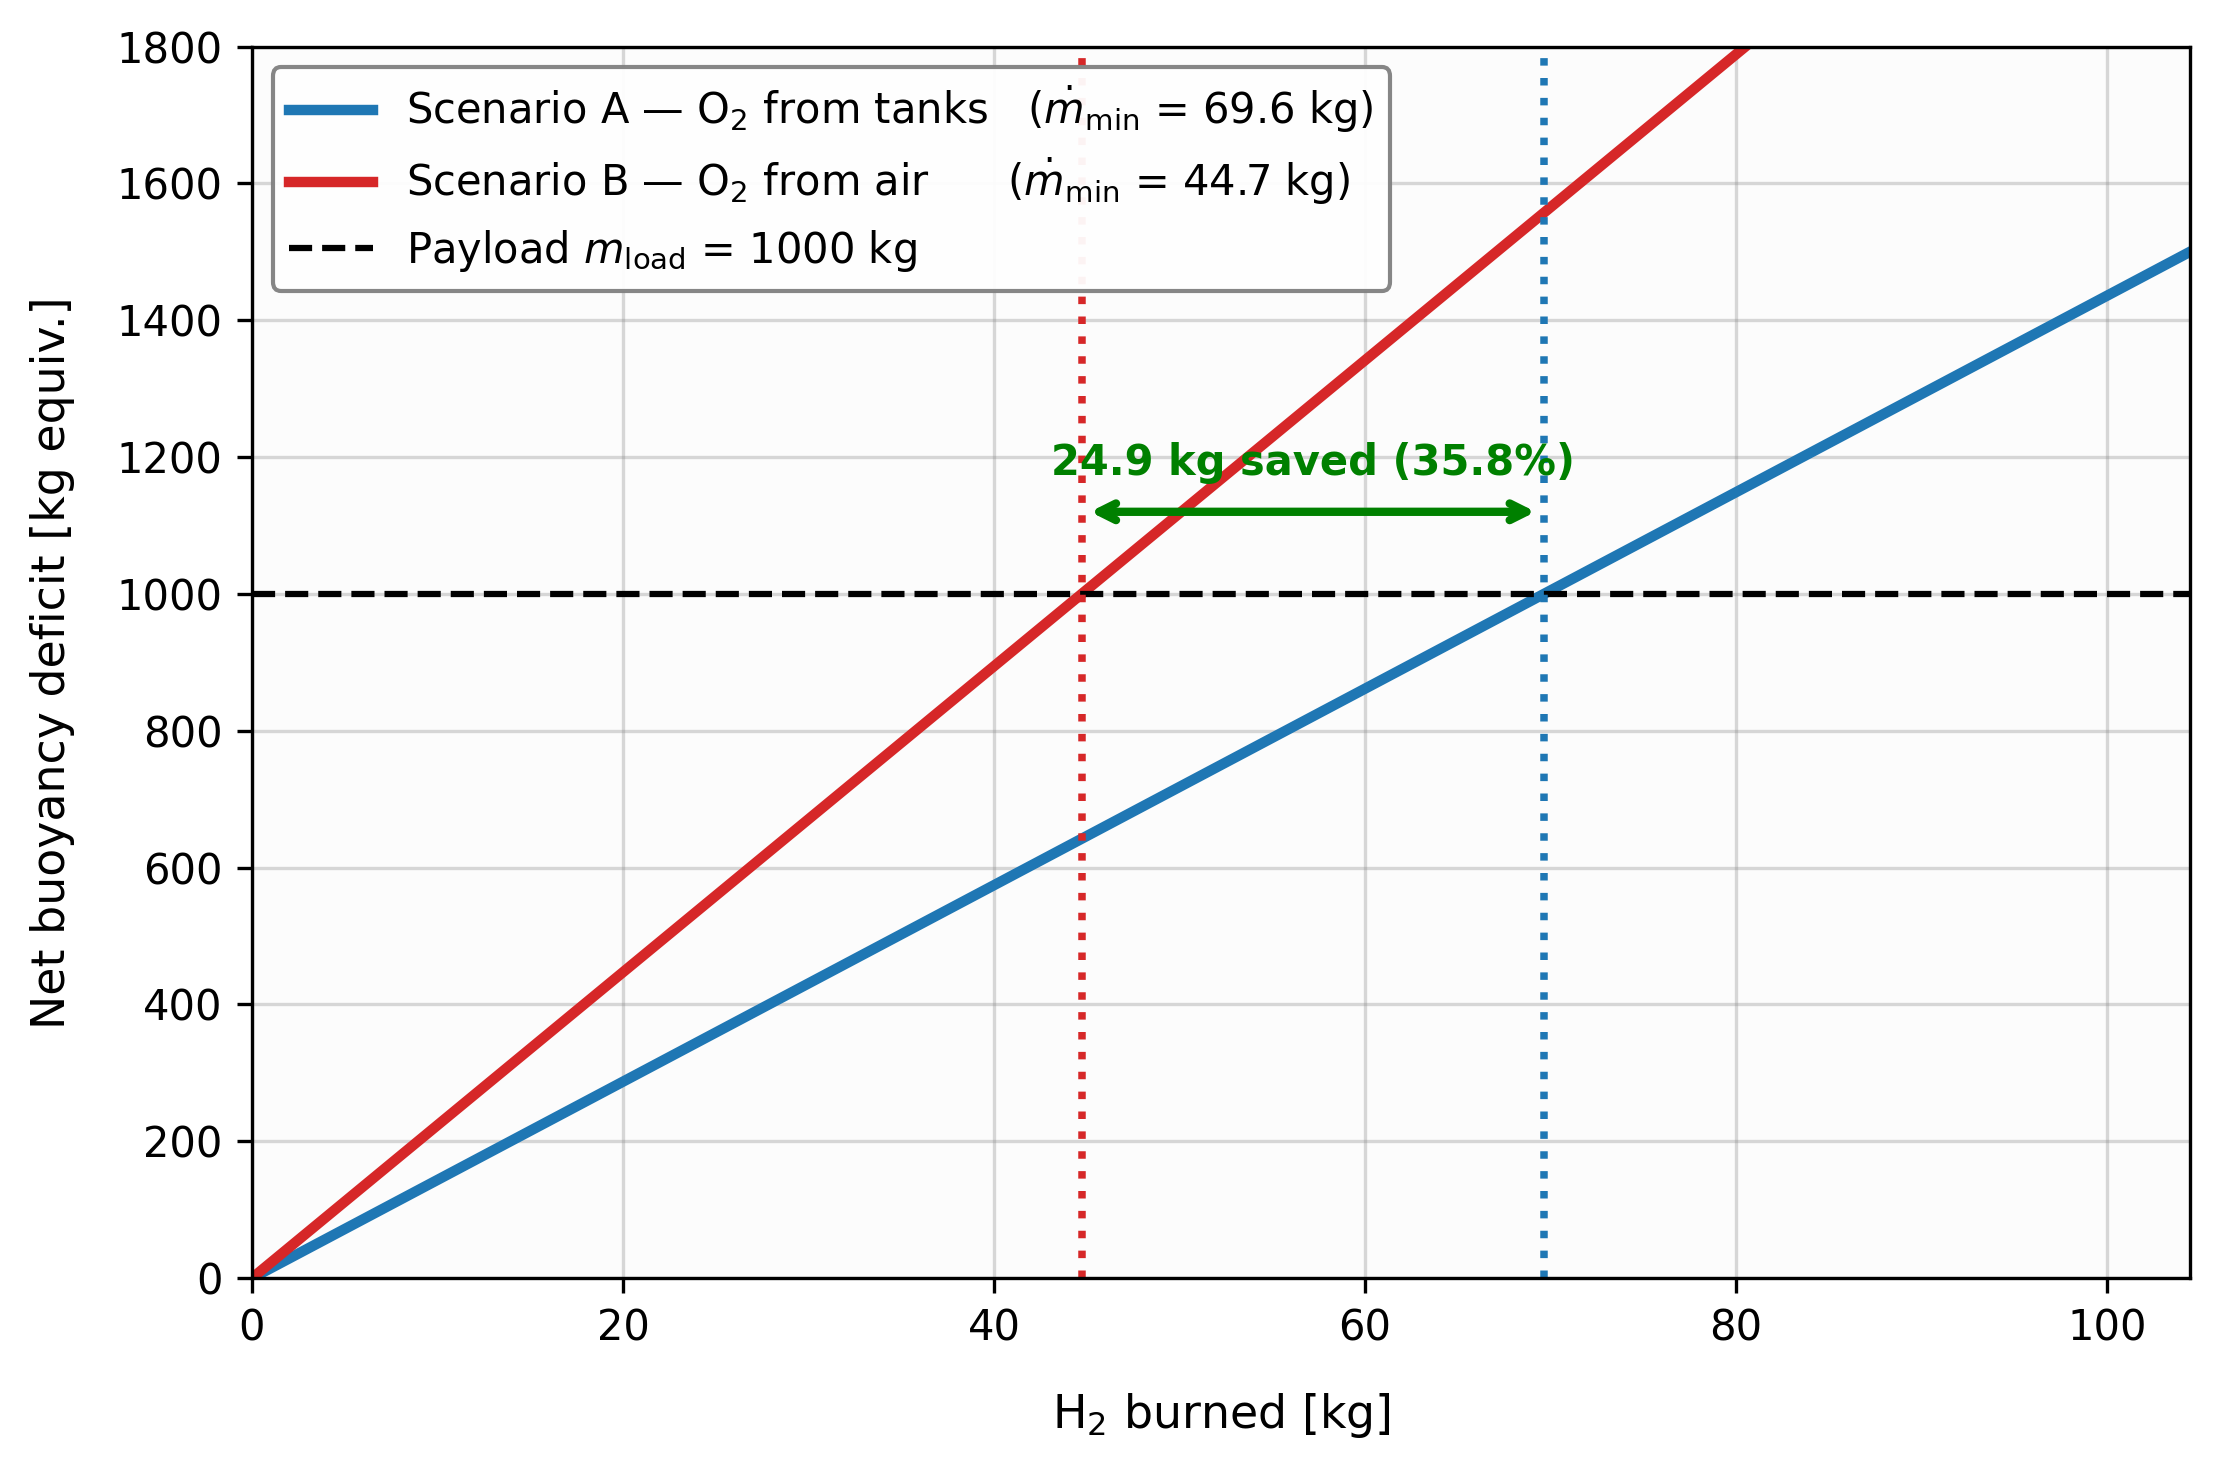
\includegraphics[width=0.9\linewidth]{buoyancy deficit.png}
\caption{Comparative analysis of the O$_2$ source (onboard tanks vs.\ atmospheric air) for the regenerative cycle after the release of 1~tonne of payload. Using atmospheric air reduces the descent-phase H$_2$ demand by ${\approx}35.8\%$ (from ${\approx}69.6$~kg to ${\approx}44.7$~kg; Eq.~\eqref{eq:mh2comb}).}
\label{fig:comparacion_o2}
\end{figure}

\subsection{Hardware Implementation Constraints}
\label{sec:combustion}
The system requires two high-power subsystems: the condenser ($Q_\text{cond,min}=1{,}512$~kW for the critical 10-min window) and the electrolysis bank. At power densities of compact brazed-aluminum heat exchangers ($\sim\!20$--$50$~kW/kg \cite{Hesselgreaves2016}), the condenser weighs between 30 and 76~kg; the PEM electrolysis bank ($\sim\!1$~kW/kg \cite{ref10}) adds approximately 84~kg to sustain one delivery cycle per day ($44.7$~kg H\textsubscript{2}/day at ${\approx}84$~kW continuous). The total hardware mass amounts to $\sim\!114$--$160$~kg, representing between 11\% and 16\% of the 1,000~kg reference payload. This penalty is critical for small airships such as the Zeppelin~NT, but becomes negligible on large-scale platforms: for the Flying Whales~LCA60T (60~t of payload) the same hardware represents less than 0.5\% of the payload capacity.

\added{Burning H\textsubscript{2} at rates of up to 50~kg/s releases thermal power on the order of 6~GW, comparable to that of liquid propellant rocket engines (the Space Shuttle's RS-25 burned ${\approx}74$~kg/s of LH\textsubscript{2} at ${\approx}3{,}300$~°C and 207~bar \cite{ref11}). However, the analogy has important limits: in the present system combustion occurs at atmospheric pressure and can be designed for continuous, low flame-temperature operation through air excess or steam dilution. Hydrogen exhibits a wide flammability range in air (4--75\% by volume \cite{Najjar2013}); safe operation is maintained through lean premix conditions ($\lambda > 2$), which reduce the adiabatic flame temperature from approximately 2{,}100~°C at stoichiometry to below 900~°C \cite{Turns2011} --- compatible with commercial high-temperature alloys and consistent with the equipment requirements established under Directive ATEX~2014/34/EU for explosive-atmosphere applications. Regenerative cooling technologies developed for rockets — where fuel preheats the chamber walls before injection — are directly transferable to this application at reduced scale, with the additional advantage that the required wall temperatures are substantially lower. The ballonet material does not come into contact with the combustion zone if it is confined in an isolated pre-chamber upstream of the heat exchanger, a standard practice in industrial H\textsubscript{2} boilers. At the nominal operating range of 4--20~kg/s, thermal power falls to 480~MW--2.4~GW.}

A higher generator efficiency ($\eta_\text{gen} \approx 0.55$, achievable with modern H\textsubscript{2} combustion systems \cite{ref9}) would not reduce H\textsubscript{2} consumption --- which depends solely on the aerostatic force balance (Eq.~\eqref{eq:mh2comb}) --- but would increase the electrical energy recovered per cycle; this improvement is directly quantifiable through Eq.~\eqref{eq:egen}, which scales linearly with $\eta_\text{gen}$. Added-mass effects \cite{Li2007} are neglected in the vertical axis model, consistent with the low accelerations involved in the controlled stabilization regime. \added{The minimax-optimal scheme introduces a hardware--fuel trade-off: reducing the installed actuator capacity from 30~kg/s to $\dotmstar = 5.21$~kg/s lowers the peak combustion hardware requirement by 83\%, but the saturated actuator operates for a longer stabilization window, increasing the total H\textsubscript{2} consumed per delivery (${\approx}96$~kg vs.\ ${\approx}46$~kg for the standard scheme; Table~\ref{tab:comparison_schemes}). The resulting higher electrolysis demand --- approximately $960$~kWh vs.\ $460$~kWh per cycle --- should be factored into solar regeneration planning when the minimax configuration is selected.}

\subsection{Future Work}
The closed-form minimax formulation of Section~\ref{sec:hybrid_bound} has been numerically validated for the Pathfinder~3 platform; its extension to the remaining three evaluated airships and to multi-axis attitude control, together with formal integration with the fine-attitude propulsion system for terminal velocity correction (Section~\ref{sec:stab_scope}), constitutes the most immediate next step. Replacing the hybrid PD scheme with a model predictive controller (MPC) that optimizes the preconditioning depth $D_\text{lim}$ and compensation fraction $\alpha^*$ in real time would extend the analytical results of Appendix~A to the closed-loop control problem. The thermomechanical design of each subsystem to satisfy the derived specifications --- condenser at $Q_\text{cond,min} \geq 1{,}512$~kW, generator sustaining $4$--$50$~kg/s, and photovoltaic array covering ${\geq}45\%$ of fuselage area --- represents the primary engineering challenge. Experimental validation at subsystem level and the definition of the \emph{ideal airship} --- the platform characteristics that simultaneously minimize all actuator, condenser, and regeneration requirements --- remain as primary directions for this research area.

%%%%%%%%%%%%%%%%%%%%%%%%%%%%%%%%%%%%%%%%%%
\section{Conclusions}

\begin{enumerate}
\item The \textbf{simulated values} range from 4~kg/s (Hindenburg) to 20~kg/s (Zeppelin~NT), within the range of existing industrial H\textsubscript{2} combustion technology (Section~\ref{sec:combustion}). The perturbation index $\varepsilon = m_\text{load}/M_\text{total}$ orders the requirements: the higher the $\varepsilon$, the higher the required rate.
\item \textbf{Larger airships are easier to stabilize}. All four evaluated airships satisfy the safety threshold ($|\Delta h| \le 5$ m) with achievable rates, with large-scale models being the most efficient.
\item \textbf{Three of the four evaluated airships} achieve energetic self-sufficiency through solar regeneration under average Lima irradiance conditions, recovering the H\textsubscript{2} consumed per delivery in less than one day. The exception is the Zeppelin~NT, whose limited surface area (2{,}800~m\textsuperscript{2}) results in a recovery cycle of approximately 30~hours (1.23~days) --- exceeding the standard 24-hour delivery cadence --- reinforcing that the regenerative cycle is naturally optimized for large-scale platforms.
\item The flow rate range $\dotmmin = 4$--$20$~kg/s is \textbf{directly actionable as a combustion subsystem specification}, with each platform's requirement ordered by the perturbation index $\varepsilon$.
\item The regenerative cycle produces a \textbf{quantifiable and predictable hydrogen demand} at a single predictable scale: ${\approx}44.7$~kg per tonne of payload (descent phase, O\textsubscript{2}-corrected), governing condenser sizing, actuator requirements, and solar regeneration planning alike. This predictability constitutes a direct input for techno-economic feasibility studies of H\textsubscript{2} supply chains in aerial heavy-lift logistics.
\item \added{The \textbf{anticipatory preconditioning strategy} reduces $\dotmmin$ below the purely-reactive analytical bound. A reactive-only approach requires ${\approx}27$~kg/s (Eq.~\eqref{eq:mmin_final}) for the smallest evaluated platform (Zeppelin~NT, $\tau_\text{ctrl} \approx 2.6$~s), while the hybrid anticipatory scheme achieves stabilization at 4--20~kg/s depending on platform inertia. The \textbf{closed-form minimax formulation} (Appendix~A) further reduces the required installed capacity to $\dotmstar = 5.21$~kg/s for the Pathfinder~3 ($\alpha^* = 0.215$, via Cardano's method) --- an $83\%$ reduction relative to the standard $30$~kg/s configuration --- by analytically optimizing the proactive compensation fraction, validated numerically within $15$--$25\%$ of the simulated values.}
\item \added{The use of \textbf{atmospheric O\textsubscript{2} as oxidizer} reduces the descent-phase H\textsubscript{2} requirement by ${\approx}36\%$ relative to an onboard-O\textsubscript{2} scheme (${\approx}44.7$ vs.\ ${\approx}70$~kg/tonne). The absorbed O\textsubscript{2} mass acts as supplementary inertial ballast during stabilization, simultaneously reducing the actuator demand and the critical-window condensation requirement, offering an additional degree of freedom for mission profile design that has no counterpart in conventional buoyancy control approaches.}
\item \added{For field implementation, the parametric analysis yields direct subsystem specifications: the condenser must provide $Q_\text{cond,min} \geq 1{,}512$~kW for the 10-min critical window (descent phase, O\textsubscript{2}-corrected); the generator unit must sustain combustion flows between 4 and 50~kg/s; and the photovoltaic array must cover at least 45\% of the fuselage surface area. Large-scale platforms such as the Pathfinder~3, Flying Whales~LCA60T, and LZ~129 Hindenburg emerge as immediate candidates for implementation, requiring ground infrastructure analogous to existing industrial H\textsubscript{2} logistics hubs.}
\end{enumerate}

%%%%%%%%%%%%%%%%%%%%%%%%%%%%%%%%%%%%%%%%%%
\vspace{6pt}

\authorcontributions{Conceptualization, A.E.L.; methodology, A.E.L.; software, A.E.L.; validation, A.E.L. and J.E.O.P.; formal analysis, A.E.L. and J.E.O.P.; investigation, A.E.L.; writing---original draft preparation, A.E.L.; writing---review and editing, J.E.O.P.; visualization, A.E.L. All authors have read and agreed to the published version of the manuscript.}

\funding{This research received no external funding.}

\dataavailability{The simulation code and datasets supporting the conclusions of this article are openly available on GitHub at \url{https://doi.org/10.5281/zenodo.19717621} and will be permanently archived in Zenodo upon acceptance. }
\conflictsofinterest{The authors declare no conflict of interest.}

\abbreviations{Abbreviations}{
The following abbreviations are used in this manuscript:\\

\noindent
\begin{tabular}{@{}ll}
$A_\text{front}$  & Frontal (aerodynamic reference) area (m$^2$) \\
$A_\text{total}$  & Total surface area of the airship (m$^2$) \\
$\alpha^*$        & Minimax-optimal proactive compensation fraction \\
$D_\text{lim}$    & Maximum allowed preconditioning sinking depth (m) \\
$h,\,\Delta h$    & Altitude and vertical displacement (m) \\
$K_p,\,K_d,\,K_m$ & Control gains (proportional, derivative, and mass) \\
$L_\text{eff}$    & Effective specific lift factor ($\rho_\text{air}/\rho_{H_2} + 8$) \\
$M_\text{str}$    & Structural mass (kg) \\
$M_\text{total}$  & Total dynamic inertial mass (kg) \\
$m_\text{load}$   & Mass of the payload to be released (kg) \\
$m_\text{water}$  & Water ballast accumulated via O$_2$ absorption (kg) \\
$\dot{m}_{H_2}$   & H$_2$ extraction/combustion rate (kg/s) \\
$\dotmmin$        & Minimum H$_2$ combustion rate for safe stabilization (kg/s) \\
$\dotmstar$       & Minimax-optimal installed actuator capacity (kg/s) \\
$\dot{m}_\text{prec}$ & Proactive preconditioning flow rate (kg/s) \\
$Q_\text{cond}$   & Condenser thermal power (kW) \\
$r_\text{ef}$     & Effective solar yield (kWh/m$^2$/day) \\
$T_1$             & Isothermal lifting gas temperature (K) \\
$t_\text{anticip}$ & Anticipation time before payload release (s) \\
$V_\text{eq}$     & Dynamic equilibrium H$_2$ volume (m$^3$) \\
$\varepsilon$     & Perturbation index ($m_\text{load}/M_\text{total}$) \\
$\eta_\text{el}$  & Electrolysis system efficiency \\
$\eta_\text{gen}$ & Effective generator efficiency \\
$\zeta$           & Adaptive damping coefficient \\
\end{tabular}
}

%%%%%%%%%%%%%%%%%%%%%%%%%%%%%%%%%%%%%%%%%%
%%%%%%%%%%%%%%%%%%%%%%%%%%%%%%%%%%%%%%%%%%
\appendix
\setcounter{section}{0}
% =============================================================================
% Appendix A — Complete Derivations: Proactive Hydrogen Preconditioning
% Included via % =============================================================================
% Appendix A — Complete Derivations: Proactive Hydrogen Preconditioning
% Included via % =============================================================================
% Appendix A — Complete Derivations: Proactive Hydrogen Preconditioning
% Included via \input{apendice_sections} after \appendix in airships_h2.tex
% NOTE: subsection titles have no manual "A.x:" prefix — MDPI cls numbers them.
% =============================================================================

\section{Complete Derivations: Proactive Hydrogen Preconditioning}
\label{sec:appendixA}

\subsection{The Cubic Formula for Pre-Drop Sinking}
\label{appx:cubic_formula}

\subsubsection{Physical Setup and Mass Definition}

Consider an airship at equilibrium altitude $h_0$ carrying a payload of mass $m_{\text{load}}$.
The lifting gas volume is $V_0$ with density $\rho_{H_2}$.
The ambient air density at altitude is $\rho_{\text{air}}$.

The total instantaneous inertial mass of the vehicle, $M_{\text{total}}$, includes the structural mass, the payload, and the mass of the hydrogen gas currently in the envelope:
\begin{equation}
  M_{\text{total}} = M_{\text{str}} + m_{\text{load}} + m_{H_2}
\end{equation}

At equilibrium (before payload release or gas extraction), the buoyant force exactly balances the total weight:
\begin{equation}
  F_{\text{buoy},0} = \rho_{\text{air}} \cdot g \cdot V_0 = M_{\text{total}} \cdot g = W_0
\end{equation}

\subsubsection{Dynamics of Hydrogen Combustion and Water Retention}

During the proactive preconditioning phase, hydrogen is transferred from the buoyancy envelope to the on-board generator at a constant mass flow rate $|\dot{m}|$.
In the generator, this hydrogen reacts with atmospheric oxygen to produce liquid water, which is retained on board as ballast.

The stoichiometric ratio dictates that 1~kg of H$_2$ reacts with approximately 8~kg of atmospheric O$_2$ to produce 9~kg of H$_2$O.
Therefore, while the envelope loses H$_2$ mass at a rate $|\dot{m}|$, the vehicle as a whole \textbf{gains} mass from the ingested oxygen at a rate $8 \cdot |\dot{m}|$.

The volume of the lifting gas as a function of time decreases linearly:
\begin{equation}
  V_{H_2}(t) = V_0 - \frac{|\dot{m}|}{\rho_{H_2}} \cdot t
\end{equation}

The total weight of the airship as a function of time \textbf{increases}:
\begin{equation}
  W(t) = \left(M_{\text{total}} + 8 \cdot |\dot{m}| \cdot t\right) \cdot g
\end{equation}

where $M_{\text{total}}$ is the initial total mass at $t = 0$ (before preconditioning begins, so
$m_{\text{water}}(0) = 0$). The increment $8|\dot{m}|t$ represents the net atmospheric O$_2$ mass
absorbed; this is identically recovered in the dynamic simulation notation of
Section~\ref{sec:methods} as $m_\text{water}(t) - |\dot{m}|t = 9|\dot{m}|t - |\dot{m}|t = 8|\dot{m}|t$,
where $m_\text{water}(t) = 9|\dot{m}|t$ is the cumulative water ballast and $|\dot{m}|t$ is the
H$_2$ mass removed from the envelope.

The net vertical force $\Delta F(t)$ acting on the airship is the difference between the instantaneous buoyancy and the instantaneous weight.
\textit{Remark}: Aerodynamic drag is neglected throughout the maneuver.
During the preconditioning phase, drag opposes the downward velocity, reducing
the actual sinking below Eq.~(\ref{eq:cubic}). During the post-release ascent,
drag opposes the upward velocity, reducing the residual buoyancy excursion and
therefore the reactive flow demand. In both phases the drag contribution is
favorable; the drag-free model provides a conservative upper bound on actuator
requirements in each phase independently.
\begin{equation}
  \Delta F(t) = \rho_{\text{air}} \cdot g \cdot V_{H_2}(t) - W(t)
\end{equation}

Substituting the time-dependent expressions:
\begin{equation}
  \Delta F(t) = \rho_{\text{air}} \cdot g \cdot \left( V_0 - \frac{|\dot{m}|}{\rho_{H_2}} \cdot t \right) - \left( M_{\text{total}} \cdot g + 8 \cdot |\dot{m}| \cdot g \cdot t \right)
\end{equation}

Since the initial equilibrium condition dictates that $\rho_{\text{air}} \cdot g \cdot V_0 = M_{\text{total}} \cdot g$, these terms cancel out:
\begin{equation}
  \Delta F(t) = - \left( \frac{\rho_{\text{air}}}{\rho_{H_2}} + 8 \right) \cdot g \cdot |\dot{m}| \cdot t = -L_\text{eff} \cdot g \cdot |\dot{m}| \cdot t
\end{equation}

where $L_{\text{eff}} = \rho_{\text{air}}/\rho_{H_2} + 8$ is the effective specific lift factor introduced in Eq.~\eqref{eq:cubic_prec}.

\subsubsection{The Cubic Formula}

Applying Newton's second law, the vertical acceleration $a(t) \approx \Delta F(t)/M_{\text{total}}$ under the approximation $8|\dot{m}|t \ll M_{\text{total}}$ (valid for $S \equiv 8|\dot{m}|t/M_{\text{total}} < 0.3$, satisfied for typical operational timescales):

\begin{equation}
  a(t) \approx - \frac{L_{\text{eff}} \cdot g \cdot |\dot{m}|}{M_{\text{total}}} \cdot t
\end{equation}

Integrating twice with initial conditions $v(0)=0$, $\Delta h(0)=0$:

\begin{equation}
  \boxed{|\Delta h(t)| = \frac{L_\text{eff}\,g\,|\dot{m}|}{6\,M_\text{total}}\,t^3}
  \label{eq:cubic}
\end{equation}

The cubic dependence arises because a constant flow rate produces a linear reduction in gas volume and a linear increase in ballast mass, both creating a linear growth in net downward force. Integrating this linear force twice yields a cubic position trajectory.

%%% -------------------------------------------------------------------
\subsection{Maximum Allowed Anticipation Time}
\label{appx:tmax_derivation}

Given that the airship cannot sink more than $D_{\max}$ before the payload is released, and defining $|\dot{m}| = \eta \cdot \dot{m}_{\text{max}}$, setting $|\Delta h(t_{\max})| = D_{\max}$ and solving:

\begin{equation}
  \boxed{t_{\max}(\eta, D_{\max}) = \left(\frac{6 \cdot M_{\text{total}} \cdot D_{\max}}{L_{\text{eff}} \cdot g \cdot \eta \cdot \dot{m}_{\text{max}}}\right)^{1/3}}
\end{equation}

%%% -------------------------------------------------------------------
\subsection{Optimal Sinking Distance for Perfect Compensation}
\label{appx:dstar_derivation}

Perfect compensation ($\alpha = 100\%$) occurs when the net downward force generated during preconditioning exactly equals the weight of the payload to be released.
The mass of hydrogen that must be burned to neutralize a payload $m_{\text{load}}$ is:
\begin{equation}
  \Delta m_{\text{pre}}^* = \frac{m_{\text{load}}}{L_{\text{eff}}}
\end{equation}

Setting $t_{\text{anticip}} = \tau \cdot t_{\max}$, with $\tau = 1$ (full available anticipation window adopted throughout), and equating to $\Delta m_{\text{pre}}^*$, then cubing and solving for $D_{\max}^*$:

\begin{equation}
  \boxed{D_{\max}^* = \frac{m_{\text{load}}^3 \cdot g}{6 \cdot M_{\text{total}} \cdot L_{\text{eff}}^2 \cdot \eta^2 \cdot \dot{m}_{\text{max}}^2 \cdot \tau^3}}
\end{equation}

%%% -------------------------------------------------------------------
\subsection{Compensation Fraction as Function of Sinking}
\label{appx:alpha_derivation}

The compensation fraction $\alpha$ is defined as the mass actually burned divided by the mass required for perfect compensation:
\begin{equation}
  \alpha = \frac{\Delta m_{\text{pre}}}{m_{\text{load}} / L_{\text{eff}}}
\end{equation}

Dividing the expression for $\Delta m_{\text{pre}}$ at arbitrary depth $D_{\max}$ by the expression at perfect compensation $D_{\max}^*$, all parameters except the distances cancel:

\begin{equation}
  \boxed{\alpha(D_{\max}) = \left(\frac{D_{\max}}{D_{\max}^*}\right)^{1/3}}
\end{equation}

%%% -------------------------------------------------------------------
\subsection{Minimum Flow Requirement for Viability}
\label{appx:mmin_viability}

If the operational sinking is limited to $D_{\text{lim}}$ and a target compensation $\alpha_{\text{target}}$ is required, substituting $D_{\text{lim}} = \alpha_{\text{target}}^3 \cdot D_{\max}^*$ into the expression for $D_{\max}^*$ and solving for $\dot{m}_{\text{max}}$:

\begin{equation}
  \boxed{\dot{m}_{\text{min}} = \frac{m_{\text{load}}^{3/2} \cdot g^{1/2} \cdot \alpha_{\text{target}}^{3/2}}{\sqrt{6 \cdot M_{\text{total}} \cdot L_{\text{eff}}^2 \cdot D_{\text{lim}}} \cdot \eta \cdot \tau^{3/2}}}
\end{equation}

For perfect compensation ($\alpha_{\text{target}} = 1$):
\begin{equation}
  \boxed{\dot{m}_{\text{min}}^{\text{pre-comp}} = \frac{m_{\text{load}}^{3/2} \cdot \sqrt{g}}{\eta \cdot \tau^{3/2} \cdot \sqrt{6 \cdot M_{\text{total}} \cdot L_{\text{eff}}^2 \cdot D_{\text{lim}}}}}
\end{equation}

\textbf{Key result}: for a fixed operational sinking limit $D_{\text{lim}}$, the minimum required flow scales inversely with the square root of the total inertial mass, recovering the scaling paradox of Eq.~\eqref{eq:mmin_final}:
\begin{equation}
  \dot{m}_{\text{min}} \propto \frac{m_{\text{load}}^{3/2}}{\sqrt{M_{\text{total}}}}
\end{equation}

%%% -------------------------------------------------------------------
\subsection{System-Level Actuator Optimization (Minimax Formulation)}
\label{appx:system_optimization}

Since both the proactive preconditioning and the reactive post-drop stabilization share the same combustion hardware, the installed capacity $\dot{m}_{\text{max}}$ must satisfy the peak demand of the more intensive phase. From Appendix~\ref{appx:mmin_viability}, the proactive demand scales as $\dot{m}_{\text{pre}}(\alpha) = K_{\text{pre}} \cdot \alpha^{3/2}$ (monotonically increasing), while the reactive demand scales as $\dot{m}_{\text{post}}(\alpha) = \dot{m}_{\text{post},0} \cdot (1-\alpha)$ (monotonically decreasing). The optimal installed capacity minimizes the peak of both:

\begin{equation}
  \dot{m}_{H_2}^* = \min_{\alpha \in [0,1]} \Bigl(\max\bigl(\dot{m}_{\text{pre}}(\alpha),\,\dot{m}_{\text{post}}(\alpha)\bigr)\Bigr)
\end{equation}

The minimum occurs at the intersection $\dot{m}_{\text{pre}}(\alpha^*) = \dot{m}_{\text{post}}(\alpha^*)$. Introducing the non-dimensional system constant:
\begin{equation}
  C = \frac{\dot{m}_{\text{post},0} \cdot \eta \cdot \tau^{3/2} \cdot \sqrt{6 \cdot M_{\text{total}} \cdot L_{\text{eff}}^2 \cdot D_{\text{lim}}}}{m_{\text{load}}^{3/2} \cdot \sqrt{g}}
\end{equation}

the change of variables $x = \sqrt{\alpha^*}$ transforms the fixed-point equation into the cubic $x^3 + C x^2 - C = 0$, which has exactly one strictly positive real root by Descartes' Rule of Signs. The exact closed-form solution depends on the discriminant $\Delta = C^2/4 - C^4/27$:

\textbf{High-inertia regime} ($\Delta > 0$, i.e., $C < 3\sqrt{3}/2$): unique real root via Cardano's method:
\begin{equation}
  \alpha^* = \left( \sqrt[3]{ \frac{C}{2} - \frac{C^3}{27} + \frac{C}{2}\sqrt{1 - \frac{4C^2}{27}} } + \sqrt[3]{ \frac{C}{2} - \frac{C^3}{27} - \frac{C}{2}\sqrt{1 - \frac{4C^2}{27}} } - \frac{C}{3} \right)^2
\end{equation}

\textbf{Low-inertia regime} ($\Delta \leq 0$, i.e., $C \geq 3\sqrt{3}/2$): three real roots (\textit{Casus Irreducibilis}); the unique physical root via Vieta's trigonometric substitution ($k=0$):
\begin{equation}
  \alpha^* = \left( \frac{2C}{3} \cos\!\left( \frac{1}{3} \arccos\!\left( \frac{27 - 2C^2}{2C^2} \right) \right) - \frac{C}{3} \right)^2
\end{equation}

These closed-form expressions eliminate the need for numerical root-finding in the actuator sizing phase and directly yield the minimax-optimal preconditioning fraction $\alpha^*$ and installed capacity $\dot{m}_{H_2}^*$ for any given airship geometry and payload configuration.
 after \appendix in airships_h2.tex
% NOTE: subsection titles have no manual "A.x:" prefix — MDPI cls numbers them.
% =============================================================================

\section{Complete Derivations: Proactive Hydrogen Preconditioning}
\label{sec:appendixA}

\subsection{The Cubic Formula for Pre-Drop Sinking}
\label{appx:cubic_formula}

\subsubsection{Physical Setup and Mass Definition}

Consider an airship at equilibrium altitude $h_0$ carrying a payload of mass $m_{\text{load}}$.
The lifting gas volume is $V_0$ with density $\rho_{H_2}$.
The ambient air density at altitude is $\rho_{\text{air}}$.

The total instantaneous inertial mass of the vehicle, $M_{\text{total}}$, includes the structural mass, the payload, and the mass of the hydrogen gas currently in the envelope:
\begin{equation}
  M_{\text{total}} = M_{\text{str}} + m_{\text{load}} + m_{H_2}
\end{equation}

At equilibrium (before payload release or gas extraction), the buoyant force exactly balances the total weight:
\begin{equation}
  F_{\text{buoy},0} = \rho_{\text{air}} \cdot g \cdot V_0 = M_{\text{total}} \cdot g = W_0
\end{equation}

\subsubsection{Dynamics of Hydrogen Combustion and Water Retention}

During the proactive preconditioning phase, hydrogen is transferred from the buoyancy envelope to the on-board generator at a constant mass flow rate $|\dot{m}|$.
In the generator, this hydrogen reacts with atmospheric oxygen to produce liquid water, which is retained on board as ballast.

The stoichiometric ratio dictates that 1~kg of H$_2$ reacts with approximately 8~kg of atmospheric O$_2$ to produce 9~kg of H$_2$O.
Therefore, while the envelope loses H$_2$ mass at a rate $|\dot{m}|$, the vehicle as a whole \textbf{gains} mass from the ingested oxygen at a rate $8 \cdot |\dot{m}|$.

The volume of the lifting gas as a function of time decreases linearly:
\begin{equation}
  V_{H_2}(t) = V_0 - \frac{|\dot{m}|}{\rho_{H_2}} \cdot t
\end{equation}

The total weight of the airship as a function of time \textbf{increases}:
\begin{equation}
  W(t) = \left(M_{\text{total}} + 8 \cdot |\dot{m}| \cdot t\right) \cdot g
\end{equation}

where $M_{\text{total}}$ is the initial total mass at $t = 0$ (before preconditioning begins, so
$m_{\text{water}}(0) = 0$). The increment $8|\dot{m}|t$ represents the net atmospheric O$_2$ mass
absorbed; this is identically recovered in the dynamic simulation notation of
Section~\ref{sec:methods} as $m_\text{water}(t) - |\dot{m}|t = 9|\dot{m}|t - |\dot{m}|t = 8|\dot{m}|t$,
where $m_\text{water}(t) = 9|\dot{m}|t$ is the cumulative water ballast and $|\dot{m}|t$ is the
H$_2$ mass removed from the envelope.

The net vertical force $\Delta F(t)$ acting on the airship is the difference between the instantaneous buoyancy and the instantaneous weight.
\textit{Remark}: Aerodynamic drag is neglected throughout the maneuver.
During the preconditioning phase, drag opposes the downward velocity, reducing
the actual sinking below Eq.~(\ref{eq:cubic}). During the post-release ascent,
drag opposes the upward velocity, reducing the residual buoyancy excursion and
therefore the reactive flow demand. In both phases the drag contribution is
favorable; the drag-free model provides a conservative upper bound on actuator
requirements in each phase independently.
\begin{equation}
  \Delta F(t) = \rho_{\text{air}} \cdot g \cdot V_{H_2}(t) - W(t)
\end{equation}

Substituting the time-dependent expressions:
\begin{equation}
  \Delta F(t) = \rho_{\text{air}} \cdot g \cdot \left( V_0 - \frac{|\dot{m}|}{\rho_{H_2}} \cdot t \right) - \left( M_{\text{total}} \cdot g + 8 \cdot |\dot{m}| \cdot g \cdot t \right)
\end{equation}

Since the initial equilibrium condition dictates that $\rho_{\text{air}} \cdot g \cdot V_0 = M_{\text{total}} \cdot g$, these terms cancel out:
\begin{equation}
  \Delta F(t) = - \left( \frac{\rho_{\text{air}}}{\rho_{H_2}} + 8 \right) \cdot g \cdot |\dot{m}| \cdot t = -L_\text{eff} \cdot g \cdot |\dot{m}| \cdot t
\end{equation}

where $L_{\text{eff}} = \rho_{\text{air}}/\rho_{H_2} + 8$ is the effective specific lift factor introduced in Eq.~\eqref{eq:cubic_prec}.

\subsubsection{The Cubic Formula}

Applying Newton's second law, the vertical acceleration $a(t) \approx \Delta F(t)/M_{\text{total}}$ under the approximation $8|\dot{m}|t \ll M_{\text{total}}$ (valid for $S \equiv 8|\dot{m}|t/M_{\text{total}} < 0.3$, satisfied for typical operational timescales):

\begin{equation}
  a(t) \approx - \frac{L_{\text{eff}} \cdot g \cdot |\dot{m}|}{M_{\text{total}}} \cdot t
\end{equation}

Integrating twice with initial conditions $v(0)=0$, $\Delta h(0)=0$:

\begin{equation}
  \boxed{|\Delta h(t)| = \frac{L_\text{eff}\,g\,|\dot{m}|}{6\,M_\text{total}}\,t^3}
  \label{eq:cubic}
\end{equation}

The cubic dependence arises because a constant flow rate produces a linear reduction in gas volume and a linear increase in ballast mass, both creating a linear growth in net downward force. Integrating this linear force twice yields a cubic position trajectory.

%%% -------------------------------------------------------------------
\subsection{Maximum Allowed Anticipation Time}
\label{appx:tmax_derivation}

Given that the airship cannot sink more than $D_{\max}$ before the payload is released, and defining $|\dot{m}| = \eta \cdot \dot{m}_{\text{max}}$, setting $|\Delta h(t_{\max})| = D_{\max}$ and solving:

\begin{equation}
  \boxed{t_{\max}(\eta, D_{\max}) = \left(\frac{6 \cdot M_{\text{total}} \cdot D_{\max}}{L_{\text{eff}} \cdot g \cdot \eta \cdot \dot{m}_{\text{max}}}\right)^{1/3}}
\end{equation}

%%% -------------------------------------------------------------------
\subsection{Optimal Sinking Distance for Perfect Compensation}
\label{appx:dstar_derivation}

Perfect compensation ($\alpha = 100\%$) occurs when the net downward force generated during preconditioning exactly equals the weight of the payload to be released.
The mass of hydrogen that must be burned to neutralize a payload $m_{\text{load}}$ is:
\begin{equation}
  \Delta m_{\text{pre}}^* = \frac{m_{\text{load}}}{L_{\text{eff}}}
\end{equation}

Setting $t_{\text{anticip}} = \tau \cdot t_{\max}$, with $\tau = 1$ (full available anticipation window adopted throughout), and equating to $\Delta m_{\text{pre}}^*$, then cubing and solving for $D_{\max}^*$:

\begin{equation}
  \boxed{D_{\max}^* = \frac{m_{\text{load}}^3 \cdot g}{6 \cdot M_{\text{total}} \cdot L_{\text{eff}}^2 \cdot \eta^2 \cdot \dot{m}_{\text{max}}^2 \cdot \tau^3}}
\end{equation}

%%% -------------------------------------------------------------------
\subsection{Compensation Fraction as Function of Sinking}
\label{appx:alpha_derivation}

The compensation fraction $\alpha$ is defined as the mass actually burned divided by the mass required for perfect compensation:
\begin{equation}
  \alpha = \frac{\Delta m_{\text{pre}}}{m_{\text{load}} / L_{\text{eff}}}
\end{equation}

Dividing the expression for $\Delta m_{\text{pre}}$ at arbitrary depth $D_{\max}$ by the expression at perfect compensation $D_{\max}^*$, all parameters except the distances cancel:

\begin{equation}
  \boxed{\alpha(D_{\max}) = \left(\frac{D_{\max}}{D_{\max}^*}\right)^{1/3}}
\end{equation}

%%% -------------------------------------------------------------------
\subsection{Minimum Flow Requirement for Viability}
\label{appx:mmin_viability}

If the operational sinking is limited to $D_{\text{lim}}$ and a target compensation $\alpha_{\text{target}}$ is required, substituting $D_{\text{lim}} = \alpha_{\text{target}}^3 \cdot D_{\max}^*$ into the expression for $D_{\max}^*$ and solving for $\dot{m}_{\text{max}}$:

\begin{equation}
  \boxed{\dot{m}_{\text{min}} = \frac{m_{\text{load}}^{3/2} \cdot g^{1/2} \cdot \alpha_{\text{target}}^{3/2}}{\sqrt{6 \cdot M_{\text{total}} \cdot L_{\text{eff}}^2 \cdot D_{\text{lim}}} \cdot \eta \cdot \tau^{3/2}}}
\end{equation}

For perfect compensation ($\alpha_{\text{target}} = 1$):
\begin{equation}
  \boxed{\dot{m}_{\text{min}}^{\text{pre-comp}} = \frac{m_{\text{load}}^{3/2} \cdot \sqrt{g}}{\eta \cdot \tau^{3/2} \cdot \sqrt{6 \cdot M_{\text{total}} \cdot L_{\text{eff}}^2 \cdot D_{\text{lim}}}}}
\end{equation}

\textbf{Key result}: for a fixed operational sinking limit $D_{\text{lim}}$, the minimum required flow scales inversely with the square root of the total inertial mass, recovering the scaling paradox of Eq.~\eqref{eq:mmin_final}:
\begin{equation}
  \dot{m}_{\text{min}} \propto \frac{m_{\text{load}}^{3/2}}{\sqrt{M_{\text{total}}}}
\end{equation}

%%% -------------------------------------------------------------------
\subsection{System-Level Actuator Optimization (Minimax Formulation)}
\label{appx:system_optimization}

Since both the proactive preconditioning and the reactive post-drop stabilization share the same combustion hardware, the installed capacity $\dot{m}_{\text{max}}$ must satisfy the peak demand of the more intensive phase. From Appendix~\ref{appx:mmin_viability}, the proactive demand scales as $\dot{m}_{\text{pre}}(\alpha) = K_{\text{pre}} \cdot \alpha^{3/2}$ (monotonically increasing), while the reactive demand scales as $\dot{m}_{\text{post}}(\alpha) = \dot{m}_{\text{post},0} \cdot (1-\alpha)$ (monotonically decreasing). The optimal installed capacity minimizes the peak of both:

\begin{equation}
  \dot{m}_{H_2}^* = \min_{\alpha \in [0,1]} \Bigl(\max\bigl(\dot{m}_{\text{pre}}(\alpha),\,\dot{m}_{\text{post}}(\alpha)\bigr)\Bigr)
\end{equation}

The minimum occurs at the intersection $\dot{m}_{\text{pre}}(\alpha^*) = \dot{m}_{\text{post}}(\alpha^*)$. Introducing the non-dimensional system constant:
\begin{equation}
  C = \frac{\dot{m}_{\text{post},0} \cdot \eta \cdot \tau^{3/2} \cdot \sqrt{6 \cdot M_{\text{total}} \cdot L_{\text{eff}}^2 \cdot D_{\text{lim}}}}{m_{\text{load}}^{3/2} \cdot \sqrt{g}}
\end{equation}

the change of variables $x = \sqrt{\alpha^*}$ transforms the fixed-point equation into the cubic $x^3 + C x^2 - C = 0$, which has exactly one strictly positive real root by Descartes' Rule of Signs. The exact closed-form solution depends on the discriminant $\Delta = C^2/4 - C^4/27$:

\textbf{High-inertia regime} ($\Delta > 0$, i.e., $C < 3\sqrt{3}/2$): unique real root via Cardano's method:
\begin{equation}
  \alpha^* = \left( \sqrt[3]{ \frac{C}{2} - \frac{C^3}{27} + \frac{C}{2}\sqrt{1 - \frac{4C^2}{27}} } + \sqrt[3]{ \frac{C}{2} - \frac{C^3}{27} - \frac{C}{2}\sqrt{1 - \frac{4C^2}{27}} } - \frac{C}{3} \right)^2
\end{equation}

\textbf{Low-inertia regime} ($\Delta \leq 0$, i.e., $C \geq 3\sqrt{3}/2$): three real roots (\textit{Casus Irreducibilis}); the unique physical root via Vieta's trigonometric substitution ($k=0$):
\begin{equation}
  \alpha^* = \left( \frac{2C}{3} \cos\!\left( \frac{1}{3} \arccos\!\left( \frac{27 - 2C^2}{2C^2} \right) \right) - \frac{C}{3} \right)^2
\end{equation}

These closed-form expressions eliminate the need for numerical root-finding in the actuator sizing phase and directly yield the minimax-optimal preconditioning fraction $\alpha^*$ and installed capacity $\dot{m}_{H_2}^*$ for any given airship geometry and payload configuration.
 after \appendix in airships_h2.tex
% NOTE: subsection titles have no manual "A.x:" prefix — MDPI cls numbers them.
% =============================================================================

\section{Complete Derivations: Proactive Hydrogen Preconditioning}
\label{sec:appendixA}

\subsection{The Cubic Formula for Pre-Drop Sinking}
\label{appx:cubic_formula}

\subsubsection{Physical Setup and Mass Definition}

Consider an airship at equilibrium altitude $h_0$ carrying a payload of mass $m_{\text{load}}$.
The lifting gas volume is $V_0$ with density $\rho_{H_2}$.
The ambient air density at altitude is $\rho_{\text{air}}$.

The total instantaneous inertial mass of the vehicle, $M_{\text{total}}$, includes the structural mass, the payload, and the mass of the hydrogen gas currently in the envelope:
\begin{equation}
  M_{\text{total}} = M_{\text{str}} + m_{\text{load}} + m_{H_2}
\end{equation}

At equilibrium (before payload release or gas extraction), the buoyant force exactly balances the total weight:
\begin{equation}
  F_{\text{buoy},0} = \rho_{\text{air}} \cdot g \cdot V_0 = M_{\text{total}} \cdot g = W_0
\end{equation}

\subsubsection{Dynamics of Hydrogen Combustion and Water Retention}

During the proactive preconditioning phase, hydrogen is transferred from the buoyancy envelope to the on-board generator at a constant mass flow rate $|\dot{m}|$.
In the generator, this hydrogen reacts with atmospheric oxygen to produce liquid water, which is retained on board as ballast.

The stoichiometric ratio dictates that 1~kg of H$_2$ reacts with approximately 8~kg of atmospheric O$_2$ to produce 9~kg of H$_2$O.
Therefore, while the envelope loses H$_2$ mass at a rate $|\dot{m}|$, the vehicle as a whole \textbf{gains} mass from the ingested oxygen at a rate $8 \cdot |\dot{m}|$.

The volume of the lifting gas as a function of time decreases linearly:
\begin{equation}
  V_{H_2}(t) = V_0 - \frac{|\dot{m}|}{\rho_{H_2}} \cdot t
\end{equation}

The total weight of the airship as a function of time \textbf{increases}:
\begin{equation}
  W(t) = \left(M_{\text{total}} + 8 \cdot |\dot{m}| \cdot t\right) \cdot g
\end{equation}

where $M_{\text{total}}$ is the initial total mass at $t = 0$ (before preconditioning begins, so
$m_{\text{water}}(0) = 0$). The increment $8|\dot{m}|t$ represents the net atmospheric O$_2$ mass
absorbed; this is identically recovered in the dynamic simulation notation of
Section~\ref{sec:methods} as $m_\text{water}(t) - |\dot{m}|t = 9|\dot{m}|t - |\dot{m}|t = 8|\dot{m}|t$,
where $m_\text{water}(t) = 9|\dot{m}|t$ is the cumulative water ballast and $|\dot{m}|t$ is the
H$_2$ mass removed from the envelope.

The net vertical force $\Delta F(t)$ acting on the airship is the difference between the instantaneous buoyancy and the instantaneous weight.
\textit{Remark}: Aerodynamic drag is neglected throughout the maneuver.
During the preconditioning phase, drag opposes the downward velocity, reducing
the actual sinking below Eq.~(\ref{eq:cubic}). During the post-release ascent,
drag opposes the upward velocity, reducing the residual buoyancy excursion and
therefore the reactive flow demand. In both phases the drag contribution is
favorable; the drag-free model provides a conservative upper bound on actuator
requirements in each phase independently.
\begin{equation}
  \Delta F(t) = \rho_{\text{air}} \cdot g \cdot V_{H_2}(t) - W(t)
\end{equation}

Substituting the time-dependent expressions:
\begin{equation}
  \Delta F(t) = \rho_{\text{air}} \cdot g \cdot \left( V_0 - \frac{|\dot{m}|}{\rho_{H_2}} \cdot t \right) - \left( M_{\text{total}} \cdot g + 8 \cdot |\dot{m}| \cdot g \cdot t \right)
\end{equation}

Since the initial equilibrium condition dictates that $\rho_{\text{air}} \cdot g \cdot V_0 = M_{\text{total}} \cdot g$, these terms cancel out:
\begin{equation}
  \Delta F(t) = - \left( \frac{\rho_{\text{air}}}{\rho_{H_2}} + 8 \right) \cdot g \cdot |\dot{m}| \cdot t = -L_\text{eff} \cdot g \cdot |\dot{m}| \cdot t
\end{equation}

where $L_{\text{eff}} = \rho_{\text{air}}/\rho_{H_2} + 8$ is the effective specific lift factor introduced in Eq.~\eqref{eq:cubic_prec}.

\subsubsection{The Cubic Formula}

Applying Newton's second law, the vertical acceleration $a(t) \approx \Delta F(t)/M_{\text{total}}$ under the approximation $8|\dot{m}|t \ll M_{\text{total}}$ (valid for $S \equiv 8|\dot{m}|t/M_{\text{total}} < 0.3$, satisfied for typical operational timescales):

\begin{equation}
  a(t) \approx - \frac{L_{\text{eff}} \cdot g \cdot |\dot{m}|}{M_{\text{total}}} \cdot t
\end{equation}

Integrating twice with initial conditions $v(0)=0$, $\Delta h(0)=0$:

\begin{equation}
  \boxed{|\Delta h(t)| = \frac{L_\text{eff}\,g\,|\dot{m}|}{6\,M_\text{total}}\,t^3}
  \label{eq:cubic}
\end{equation}

The cubic dependence arises because a constant flow rate produces a linear reduction in gas volume and a linear increase in ballast mass, both creating a linear growth in net downward force. Integrating this linear force twice yields a cubic position trajectory.

%%% -------------------------------------------------------------------
\subsection{Maximum Allowed Anticipation Time}
\label{appx:tmax_derivation}

Given that the airship cannot sink more than $D_{\max}$ before the payload is released, and defining $|\dot{m}| = \eta \cdot \dot{m}_{\text{max}}$, setting $|\Delta h(t_{\max})| = D_{\max}$ and solving:

\begin{equation}
  \boxed{t_{\max}(\eta, D_{\max}) = \left(\frac{6 \cdot M_{\text{total}} \cdot D_{\max}}{L_{\text{eff}} \cdot g \cdot \eta \cdot \dot{m}_{\text{max}}}\right)^{1/3}}
\end{equation}

%%% -------------------------------------------------------------------
\subsection{Optimal Sinking Distance for Perfect Compensation}
\label{appx:dstar_derivation}

Perfect compensation ($\alpha = 100\%$) occurs when the net downward force generated during preconditioning exactly equals the weight of the payload to be released.
The mass of hydrogen that must be burned to neutralize a payload $m_{\text{load}}$ is:
\begin{equation}
  \Delta m_{\text{pre}}^* = \frac{m_{\text{load}}}{L_{\text{eff}}}
\end{equation}

Setting $t_{\text{anticip}} = \tau \cdot t_{\max}$, with $\tau = 1$ (full available anticipation window adopted throughout), and equating to $\Delta m_{\text{pre}}^*$, then cubing and solving for $D_{\max}^*$:

\begin{equation}
  \boxed{D_{\max}^* = \frac{m_{\text{load}}^3 \cdot g}{6 \cdot M_{\text{total}} \cdot L_{\text{eff}}^2 \cdot \eta^2 \cdot \dot{m}_{\text{max}}^2 \cdot \tau^3}}
\end{equation}

%%% -------------------------------------------------------------------
\subsection{Compensation Fraction as Function of Sinking}
\label{appx:alpha_derivation}

The compensation fraction $\alpha$ is defined as the mass actually burned divided by the mass required for perfect compensation:
\begin{equation}
  \alpha = \frac{\Delta m_{\text{pre}}}{m_{\text{load}} / L_{\text{eff}}}
\end{equation}

Dividing the expression for $\Delta m_{\text{pre}}$ at arbitrary depth $D_{\max}$ by the expression at perfect compensation $D_{\max}^*$, all parameters except the distances cancel:

\begin{equation}
  \boxed{\alpha(D_{\max}) = \left(\frac{D_{\max}}{D_{\max}^*}\right)^{1/3}}
\end{equation}

%%% -------------------------------------------------------------------
\subsection{Minimum Flow Requirement for Viability}
\label{appx:mmin_viability}

If the operational sinking is limited to $D_{\text{lim}}$ and a target compensation $\alpha_{\text{target}}$ is required, substituting $D_{\text{lim}} = \alpha_{\text{target}}^3 \cdot D_{\max}^*$ into the expression for $D_{\max}^*$ and solving for $\dot{m}_{\text{max}}$:

\begin{equation}
  \boxed{\dot{m}_{\text{min}} = \frac{m_{\text{load}}^{3/2} \cdot g^{1/2} \cdot \alpha_{\text{target}}^{3/2}}{\sqrt{6 \cdot M_{\text{total}} \cdot L_{\text{eff}}^2 \cdot D_{\text{lim}}} \cdot \eta \cdot \tau^{3/2}}}
\end{equation}

For perfect compensation ($\alpha_{\text{target}} = 1$):
\begin{equation}
  \boxed{\dot{m}_{\text{min}}^{\text{pre-comp}} = \frac{m_{\text{load}}^{3/2} \cdot \sqrt{g}}{\eta \cdot \tau^{3/2} \cdot \sqrt{6 \cdot M_{\text{total}} \cdot L_{\text{eff}}^2 \cdot D_{\text{lim}}}}}
\end{equation}

\textbf{Key result}: for a fixed operational sinking limit $D_{\text{lim}}$, the minimum required flow scales inversely with the square root of the total inertial mass, recovering the scaling paradox of Eq.~\eqref{eq:mmin_final}:
\begin{equation}
  \dot{m}_{\text{min}} \propto \frac{m_{\text{load}}^{3/2}}{\sqrt{M_{\text{total}}}}
\end{equation}

%%% -------------------------------------------------------------------
\subsection{System-Level Actuator Optimization (Minimax Formulation)}
\label{appx:system_optimization}

Since both the proactive preconditioning and the reactive post-drop stabilization share the same combustion hardware, the installed capacity $\dot{m}_{\text{max}}$ must satisfy the peak demand of the more intensive phase. From Appendix~\ref{appx:mmin_viability}, the proactive demand scales as $\dot{m}_{\text{pre}}(\alpha) = K_{\text{pre}} \cdot \alpha^{3/2}$ (monotonically increasing), while the reactive demand scales as $\dot{m}_{\text{post}}(\alpha) = \dot{m}_{\text{post},0} \cdot (1-\alpha)$ (monotonically decreasing). The optimal installed capacity minimizes the peak of both:

\begin{equation}
  \dot{m}_{H_2}^* = \min_{\alpha \in [0,1]} \Bigl(\max\bigl(\dot{m}_{\text{pre}}(\alpha),\,\dot{m}_{\text{post}}(\alpha)\bigr)\Bigr)
\end{equation}

The minimum occurs at the intersection $\dot{m}_{\text{pre}}(\alpha^*) = \dot{m}_{\text{post}}(\alpha^*)$. Introducing the non-dimensional system constant:
\begin{equation}
  C = \frac{\dot{m}_{\text{post},0} \cdot \eta \cdot \tau^{3/2} \cdot \sqrt{6 \cdot M_{\text{total}} \cdot L_{\text{eff}}^2 \cdot D_{\text{lim}}}}{m_{\text{load}}^{3/2} \cdot \sqrt{g}}
\end{equation}

the change of variables $x = \sqrt{\alpha^*}$ transforms the fixed-point equation into the cubic $x^3 + C x^2 - C = 0$, which has exactly one strictly positive real root by Descartes' Rule of Signs. The exact closed-form solution depends on the discriminant $\Delta = C^2/4 - C^4/27$:

\textbf{High-inertia regime} ($\Delta > 0$, i.e., $C < 3\sqrt{3}/2$): unique real root via Cardano's method:
\begin{equation}
  \alpha^* = \left( \sqrt[3]{ \frac{C}{2} - \frac{C^3}{27} + \frac{C}{2}\sqrt{1 - \frac{4C^2}{27}} } + \sqrt[3]{ \frac{C}{2} - \frac{C^3}{27} - \frac{C}{2}\sqrt{1 - \frac{4C^2}{27}} } - \frac{C}{3} \right)^2
\end{equation}

\textbf{Low-inertia regime} ($\Delta \leq 0$, i.e., $C \geq 3\sqrt{3}/2$): three real roots (\textit{Casus Irreducibilis}); the unique physical root via Vieta's trigonometric substitution ($k=0$):
\begin{equation}
  \alpha^* = \left( \frac{2C}{3} \cos\!\left( \frac{1}{3} \arccos\!\left( \frac{27 - 2C^2}{2C^2} \right) \right) - \frac{C}{3} \right)^2
\end{equation}

These closed-form expressions eliminate the need for numerical root-finding in the actuator sizing phase and directly yield the minimax-optimal preconditioning fraction $\alpha^*$ and installed capacity $\dot{m}_{H_2}^*$ for any given airship geometry and payload configuration.

\section{Adaptive PD Controller: Full Implementation}
\label{app:control}

\subsection*{Gain Scheduling}

The derivative gain is adaptively tuned to maintain a constant damping coefficient $\zeta = 1.35$ throughout the unloading sequence:

\begin{equation}
K_d(t) = 2\,\zeta\,\sqrt{\frac{K_p\,M_\text{eff}(t)}{\rho_\text{air}(h)\,g}}, \qquad
M_\text{eff}(t) = M_\text{str} + M_\text{load}(t) + m_\text{water}(t)
\label{eq:kd_app}
\end{equation}

where $M_\text{eff}$ includes the structural mass, remaining payload, and accumulated water ballast, but excludes $m_{H_2}$ (gas mass contributes to buoyancy rather than inertial damping). This expression is derived by imposing that the damping coefficient $\zeta$ of the linearized system remains constant under mass variations; without this adaptation, the step-wise loss of payload and concurrent gain of water ballast would progressively alter the dynamic regime.

\subsection*{Feedback Flow Law}

The mass flow rate commanded by the feedback controller is:

\begin{equation}
\dot{m}_\text{PD}(t) = K_m\bigl(V_\text{eq}(t) + K_p\,e_h - K_d(t)\,v - V_{H_2}\bigr)
\label{eq:mpd_app}
\end{equation}

where $e_h = h_0 - h$ is the altitude error. The gain $K_m$ operates in two sequential phases: an \emph{emergency phase} ($K_m = 60$~kg/s/m\textsuperscript{3}) provides rapid post-drop response until $m_{H_2}$ reaches the new equilibrium target $m_{H_2,\text{eq}} = M_\text{eff}/(\rho_0/\rho_{H_2}-1)$; a \emph{trim phase} ($K_m = 0.5$~kg/s/m\textsuperscript{3}) then guides smooth settling to the new equilibrium. The emergency phase ensures aggressive compensation of the initial perturbation; the reduced trim gain prevents oscillation buildup and resets automatically at each subsequent drop event.

\subsection*{Anticipatory Preconditioning}

To mitigate the initial acceleration peak, the system incorporates an anticipatory extraction pulse. Two seconds before the scheduled release instant ($t_\text{drop}$), the system temporarily suspends the PD control and injects a constant negative flow $\dot{m}_\text{prec} = -10$~kg/s. Extracting this flow for 2~seconds induces a proactive lift deficit sufficient to partially absorb the perturbation before release. With atmospheric O\textsubscript{2} as oxidizer, the absorbed fraction is governed by the effective specific lift factor $L_\text{eff}$ (Eq.~\eqref{eq:cubic_prec}), which combines buoyancy loss and absorbed O\textsubscript{2} mass:

\begin{equation}
\frac{\Delta F}{\Delta F_\text{pert}} = L_\text{eff}\cdot\frac{|\dot{m}_\text{prec}|\,t_\text{prec}}{m_\text{load}} \approx 44.8\%
\label{eq:alpha_prec_B}
\end{equation}

for the nominal parameters of Table~\ref{tab:parametros}. The buoyancy-only contribution accounts for $(\rho_\text{air}/\rho_{H_2}) \times \ldots \approx 28.8\%$; the remaining ${\approx}16\%$ is provided by the O\textsubscript{2} mass absorbed and retained as water ballast during the 2-second preconditioning window. The anticipation time $t_\text{anticip} = 2.0$~s is selected such that the resulting preconditioning sinking depth (Eq.~\eqref{eq:cubic_prec}) satisfies $D_\text{lim} \approx 0.027$~m for the Pathfinder~3 --- negligible relative to the post-drop safety threshold ($|\Delta h|_\text{max} = 5$~m) --- while providing the maximum pre-compensation consistent with this constraint.

\subsection*{Hybrid Control Law}

The hybrid control law with saturation is defined as:

\begin{equation}
\dot{m}_{H_2}(t) =
\begin{cases}
\dot{m}_\text{prec} & \text{if } t \in [t_\text{drop}-2\,\text{s},\; t_\text{drop}) \\
\text{sat}_{\dotmmax}\!\left(\dot{m}_\text{PD}(t)\right) & \text{otherwise}
\end{cases}
\label{eq:hybrid_app}
\end{equation}

This saturation at $\pm\dotmmax$ is the critical design parameter: if the hybrid scheme demands more flow than the system can provide, the vertical displacement exceeds the operational safety threshold. The proactive pulse qualitatively transforms this requirement: instead of requiring the actuator to compensate for an already-initiated upward impulse, it anticipates the perturbation by reducing net buoyancy \emph{before} the release. The PD controller then acts on a system that is already partially in descent, drastically reducing the reactive flow required.


%%%%%%%%%%%%%%%%%%%%%%%%%%%%%%%%%%%%%%%%%%
% FASE 6: bibliografía reordenada por primera aparición en texto (MDPI req.)
\begin{thebibliography}{999}
\bibitem{ref1} Prentice, B.E.; Knotts, R. Cargo Airships: International Competition. \textit{J. Transp. Technol.} \textbf{2014}, \textit{4}, 187--195. \url{https://doi.org/10.4236/jtts.2014.43019}
\bibitem{ref2} Khoury, G. A. \textit{Airship Technology}, 2nd ed.; Cambridge University Press: Cambridge, UK, 2012; ISBN 9781107019706.
\bibitem{ref4} Hybrid Air Vehicles. \textit{Airlander 10 Technical Specifications}, 2023. [Online]. \url{https://www.airlander.com/technology} [Accessed: 13 June 2026].
\bibitem{ref5} Flying Whales. \textit{LCA60T Technical Overview}, 2023. [Online]. \url{https://flying-whales.com/} [Accessed: 13 June 2026].
\bibitem{ref6} LTA Research and Exploration. \textit{Pathfinder 1 First Flight --- Program Overview}, 2023. [Online]. \url{https://ltaresearch.com/} [Accessed: 13 June 2026].
\bibitem{BenAbdallah2019} Ben Abdallah, F.; Azouz, N.; Beji, L.; Abichou, A. Modeling of a heavy-lift airship carrying a payload by a cable-driven parallel manipulator. \textit{Int. J. Adv. Robot. Syst.} \textbf{2019}, \textit{16}(4), 1--17. \url{https://doi.org/10.1177/1729881419861769}
\bibitem{Lanteigne2017} Lanteigne, E.; Alsayed, A.; Robillard, D.; Recoskie, S.G. Modeling and control of an unmanned airship with sliding ballast. \textit{J. Intell. Robot. Syst.} \textbf{2017}, \textit{88}(2--4), 285--297. \url{https://doi.org/10.1007/s10846-017-0533-6}
\bibitem{Barton2013} Barton, S.A. Airship buoyancy control using inflatable vacuum chambers. \textit{J. Aircr.} \textbf{2013}, \textit{50}(4), 1315--1317. \url{https://doi.org/10.2514/1.C031654}
\bibitem{Li2007} Li, Y.; Nahon, M. Modeling and simulation of airship dynamics. \textit{J. Guid. Control Dyn.} \textbf{2007}, \textit{30}(6), 1691--1700. \url{https://doi.org/10.2514/1.29061}
\bibitem{Pasternak2015} Pasternak, I. et al. Flight system for a constant volume, variable buoyancy air vehicle (Control of Static Heaviness --- COSH). U.S. Patent 9,016,622 B1, Worldwide Aeros Corp., 2015. \url{https://patents.google.com/patent/US9016622}
\bibitem{Sun2024} Sun, K.; Ji, X.; Shan, C.; Cheng, D.; Liang, H. Extending the flight endurance of stratospheric airships using regenerative fuel cells-assisted pressure maintenance. \textit{Renew. Energy} \textbf{2024}, \textit{227}, 120470. \url{https://doi.org/10.1016/j.renene.2024.120470}
\bibitem{Kowsari2024} Kowsari, M.; Ghabcheloo, R. Optimal sway motion reduction in forestry cranes. \textit{Front. Robot. AI} \textbf{2024}, \textit{11}, 1417741. \url{https://doi.org/10.3389/frobt.2024.1417741}
\bibitem{ref7} Federal Aviation Administration (FAA). \textit{Helicopter Flying Handbook (FAA-H-8083-21B)}. U.S. Department of Transportation, 2019.
\bibitem{ref8} Department of the Navy. \textit{NWP 4-01.4: Underway Replenishment}. U.S. Navy, 2018.
\bibitem{Schmidt2007} Schmidt, D.K. Modeling and near-space stationkeeping control of a large high-altitude airship. \textit{J. Guid. Control Dyn.} \textbf{2007}, \textit{30}(2), 540--547. \url{https://doi.org/10.2514/1.24865}
\bibitem{Liao2009} Liao, L.; Pasternak, I. A review of airship structural research and development. \textit{Prog. Aerosp. Sci.} \textbf{2009}, \textit{45}(4--5), 83--96. \url{https://doi.org/10.1016/j.paerosci.2009.03.001}
\bibitem{SAE2023} SAE International. \textit{Fueling Protocols for Medium and Heavy Duty Gaseous Hydrogen Surface Vehicles (SAE J2601-2)}; SAE International: Warrendale, PA, USA, 2023.
\bibitem{ref9} Verhelst, S.; Wallner, T. Hydrogen-fueled internal combustion engines. \textit{Prog. Energy Combust. Sci.} \textbf{2009}, \textit{35}(6), 490--527. \url{https://doi.org/10.1016/j.pecs.2009.08.001}
\bibitem{ref10} IRENA. \textit{Green Hydrogen Cost Reduction: Scaling up Electrolysers to Meet the 1.5°C Climate Goal}. International Renewable Energy Agency, Abu Dhabi, 2020.
\bibitem{Buttler2018} Buttler, A.; Spliethoff, H. Current status of water electrolysis for energy storage, grid balancing and sector coupling via power-to-gas and power-to-liquids: A review. \textit{Renew. Sustain. Energy Rev.} \textbf{2018}, \textit{82}, 2440--2454. \url{https://doi.org/10.1016/j.rser.2017.09.003}
\bibitem{Falcao2020} Falcão, D.S.; Pinto, A.M.F.R. A review on PEM electrolyzer modelling: Guidelines for beginners. \textit{J. Clean. Prod.} \textbf{2020}, \textit{261}, 121184. \url{https://doi.org/10.1016/j.jclepro.2020.121184}
\bibitem{SENAMHI2003} SENAMHI; MINEM. \textit{Atlas de Energía Solar del Perú}; SENAMHI: Lima, Peru, 2003. [Online]. \url{https://www.senamhi.gob.pe/pdf/Atlas%20_de_Radiacion_Solar.pdf} [Accessed: 13 June 2026].
\bibitem{Gao2024} Gao, X.; Hou, Z.; Zhu, X.; Chen, X. Configuration optimization of PV array for stratospheric airship under nonuniform radiation condition. \textit{Aerosp. Sci. Technol.} \textbf{2024}, \textit{154}, 109538. \url{https://doi.org/10.1016/j.ast.2024.109538}
\bibitem{Azinheira2016} Moutinho, A.; Azinheira, J.R.; de Paiva, E.C.; Bueno, S.S. Airship robust path-tracking: A tutorial on airship modelling and gain-scheduling control design. \textit{Control Eng. Pract.} \textbf{2016}, \textit{50}, 22--36. \url{https://doi.org/10.1016/j.conengprac.2016.02.009}
\bibitem{Wu2013} Wu, X.; Moog, C.H.; Márquez-Martínez, L.A.; Hu, Y. Full model of a buoyancy-driven airship and its control in the vertical plane. \textit{Aerosp. Sci. Technol.} \textbf{2013}, \textit{26}(1), 138--152. \url{https://doi.org/10.1016/j.ast.2012.02.022}
\bibitem{Zhang2019} Zhang, L.; Li, J.; Jiang, Y.; Du, H.; Zhu, W.; Lv, M. Analysis of attitude planning and energy balance of stratospheric airship. \textit{Energy} \textbf{2019}, \textit{183}, 1089--1103. \url{https://doi.org/10.1016/j.energy.2019.07.002}
\bibitem{Hesselgreaves2016} Hesselgreaves, J.E.; Law, R.; Reay, D. \textit{Compact Heat Exchangers: Selection, Design and Operation}, 2nd ed.; Elsevier Butterworth-Heinemann: Oxford, UK, 2016; ISBN 9780081003053.
\bibitem{ref11} NASA. \textit{SLS (Space Launch System) RS-25 Core Stage Engine}. NASA Marshall Space Flight Center. [Online]. \url{https://www.nasa.gov/reference/space-launch-system-rs-25-core-stage-engine/} [Accessed: 13 June 2026].
\bibitem{Najjar2013} Najjar, Y.S.H. Hydrogen safety: The road toward green technology. \textit{Int. J. Hydrogen Energy} \textbf{2013}, \textit{38}(25), 10716--10728. \url{https://doi.org/10.1016/j.ijhydene.2013.05.126}
\bibitem{Turns2011} Turns, S.R. \textit{An Introduction to Combustion: Concepts and Applications}, 3rd ed.; McGraw-Hill: New York, NY, USA, 2011.
\end{thebibliography}

\end{document}